\chapter{Algèbre linéaire}


%%%%%%%%%%%%%%%%%%%%%%%%%%%%%%%%%%%%%%%%%%%%%%%%%%%%%
\section{Opérations matricielles}
\label{sec:opmat}
%%%%%%%%%%%%%%%%%%%%%%%%%%%%%%%%%%%%%%%%%%%%%%%%%%%%%
L'algèbre linéaire, c'est à la base une collection d'outils mathématique pour traiter plusieurs fonctions/opérations en parallèle.

%%%%%%%%%%%%%%%%%%%%%%%%%%%%%%%%%%%%%%%%%%%%%%%%%%%%%
\subsection{L'opération $\col{y} = A \col{x}$}
%%%%%%%%%%%%%%%%%%%%%%%%%%%%%%%%%%%%%%%%%%%%%%%%%%%%%

 L'opération $\col{y} = A \col{x}$ est un outil mathématique pour faire $m$ opérations linéaires sur les variables $x_i$ dans le vecteur-colonne $\col{x}$. Les outils de l'algèbre linéaire sont donc particulièrement utiles pour travailler avec des quantités multivariables comme des vecteurs 3D de position, vitesse, forces, etc.

%%%%%%%%%%%%%%%%%%%%%%%%%%%%%
\begin{figure}[htbp]
	\centering
		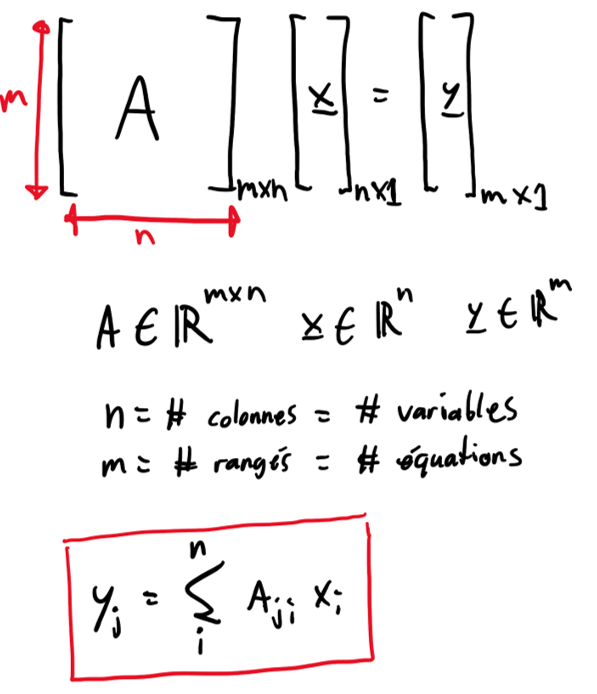
\includegraphics[width=0.50\textwidth]{calculmatriciel.png}
	\caption{L'opération matricielle $\col{y} = A \col{x}$}
	\label{fig:calculmatriciel}
\end{figure}
%%%%%%%%%%%%%%%%%%%%%%%%%%%%%

%%%%%%%%%%%%%%%%%%%%%%%%%%%%%%%%%%%%%%%%%%%%%%%%%%%%%
\subsubsection{Système d’équations}
\label{sec:syseq}
%%%%%%%%%%%%%%%%%%%%%%%%%%%%%%%%%%%%%%%%%%%%%%%%%%%%%

L'opération matricielle $\col{y} = A \col{x}$ peut d'abord être vue comme un système de $m$ équations linéaires.  Par exemple, deux fonctions linéaires, $f_1$ et $f_2$, de deux variables (entrées), $x_1$ et $x_2$, peuvent s’écrire :
%%%%%%%%%%%%%%%%%%%%%%%%%%%%%
\begin{align}
y_1 = f_1(x_1,x_2) = a_{11} \, x_1 + a_{12} \, x_2   \\
y_2 = f_2(x_1,x_2) = a_{21} \, x_1 + a_{22} \, x_2
\end{align}
%%%%%%%%%%%%%%%%%%%%%%%%%%%%%
ou $y_1$ et $y_2$ sont les variables résultats (sorties) des fonctions, et $a_{ii}$ les paramètres internes des fonctions. Ces équations, avec la notation matricielle prennent la forme:
%%%%%%%%%%%%%%%%%%%%%%%%%%%%%
\begin{align}
\left[ \begin{array}{c} 
	y_1 \\ y_2
\end{array} \right] &= 
\left[ \begin{array}{c c} 
a_{11} & a_{12} \\ a_{21} & a_{22}
\end{array} \right]
\left[ \begin{array}{c} 
	x_1 \\ x_2
\end{array} \right] \quad \leftrightarrow \quad  \col{y}  =   A  \col{x} 
\label{eq:sys2}
\end{align}
%%%%%%%%%%%%%%%%%%%%%%%%%%%%%
ou $\col{y}$ et $\col{x}$ sont des vecteur-colonnes de dimension 2 et $A$ est une matrice 2x2. De façon générale, une matrice d'un tel système d’équation a une largeur $n$, correspondant au nombre de variable dans les équations, et une hauteur $m$, correspondant au nombre d’équations.
%
\begin{align}
\left[ \begin{array}{c} 
	y_1 \\ \vdots \\ y_m
\end{array} \right] &= 
\left[ \begin{array}{c c c} 
a_{11} & ... & a_{1n} \\ \vdots & \ddots  &  \vdots \\ 
a_{m1} & ... & a_{mn}
\end{array} \right]
\left[ \begin{array}{c} 
	x_1 \\ \vdots \\ x_n
\end{array} \right] \\
m: \quad \text{nombre de ranges} \quad&=\quad \text{nombre d’équations / sorties} \\
n: \quad \text{nombre de colonnes} \quad&=\quad \text{nombre de variables / entrées}
\end{align}
%


%%%%%%%%%%%%%%%%%%%%%%%%%%%%%%%%%%%%%%%%%%%%%%%%%%%%%
\subsubsection{Combinaison de vecteur-colonnes}
\label{sec:combveccol}
%%%%%%%%%%%%%%%%%%%%%%%%%%%%%%%%%%%%%%%%%%%%%%%%%%%%%

La multiplication d'une matrice par un vecteur-colonne peut être vue comme une combinaison linéaire des vecteur-colonnes de la matrice. Cette interprétation est très importante pour comprendre toutes les propriétés importantes et utiles des matrices, qui seront détaillées dans les prochaines sections. L’équation \eqref{eq:sys2}, correspondant a la multiplication d'un vecteur-colonne de dimension 2 par une matrice $2\times2$ peut être réécrite comme l'addition pondérée des deux colonnes de la matrice:
%
\begin{align}
\left[ \begin{array}{c} 
	y_1 \\ y_2
\end{array} \right] &= 
\left[ \begin{array}{c c} 
a_{11} & a_{12} \\ a_{21} & a_{22}
\end{array} \right]
\left[ \begin{array}{c} 
	x_1 \\ x_2
\end{array} \right] \quad \leftrightarrow \quad  \col{y}  =   
%
\underbrace{\left[ \begin{array}{c} 
	a_{11} \\ a_{21}
\end{array} \right]}_{\col{c}_1} \, x_1 +
\underbrace{\left[ \begin{array}{c} 
	a_{12} \\ a_{22}
\end{array} \right]}_{\col{c}_2} \, x_2
\label{eq:sys2-col}
\end{align}
%
Graphiquement, tel illustré à la figure \ref{fig:lincomb}, la multiplication d'une matrice peux être représenté par une addition pondérée (combinaison linéaire) des vecteurs correspondants aux colonnes de la matrice, dans l'espace sortie $\col{y} \in \re^m$.

%%%%%%%%%%%%%%%%%%%%%%%%%%%%%%%%%%%%%%%%%%%%%%%%%%%%%%%%%%%%
\begin{figure}[H]
	\centering
		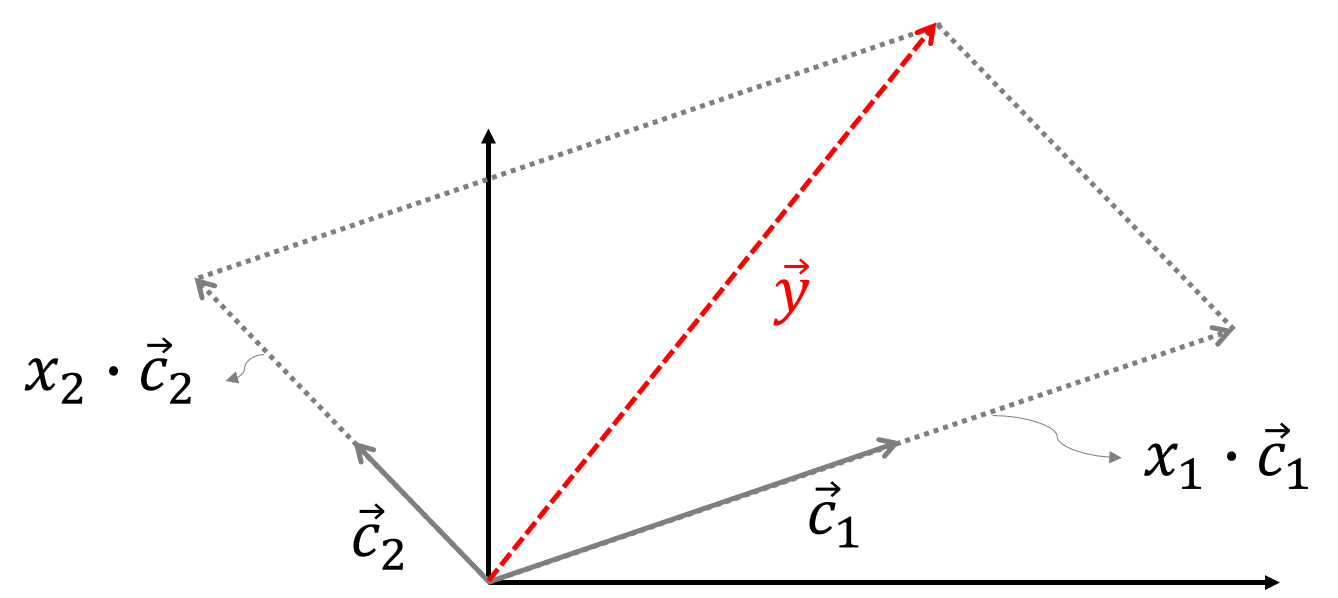
\includegraphics[width=0.60\textwidth]{lincomb.png}
	\caption{La multiplication matricielle comme une combinaison lineaire de vecteurs}
	\label{fig:lincomb}
\end{figure}
%%%%%%%%%%%%%%%%%%%%%%%%%%%%%%%%%%%%%%%%%%%%%%%%%%%%%%%%%%%%

De façon générale, le vecteur-colonne $\col{y}$ résultant d'une multiplication d'une matrice $A$ avec un vecteur-colonne $\col{x}$, peut-être exprimée comme une combinaison linéaire des colonnes de la matrice $A$:
%%%%%%%%%%%%%%%%%%%%%%
\begin{align}
%
\left[ \begin{array}{c} 
	y_1 \\ \vdots \\ y_m
\end{array} \right] 
%
&= 
%
\left[ \begin{array}{c c c c c} 
\underbrace{\left[ \begin{array}{c} 
	a_{11} \\ \vdots \\ a_{1m}
\end{array} \right]}_{\col{c}_1}
& ... &
\underbrace{\left[ \begin{array}{c} 
	a_{i1} \\ \vdots \\ a_{im}
\end{array} \right]}_{\col{c}_i}
& ... &
\underbrace{\left[ \begin{array}{c} 
	a_{n1} \\ \vdots \\ a_{nm}
\end{array} \right]}_{\col{c}_n}
\end{array} \right] 
%
\left[ \begin{array}{c} 
	x_1 \\ \vdots \\ x_n
\end{array} \right]  \\
%
%
\col{y}
&= \sum_{i=1}^{n}{ \col{c}_i x_i}
\end{align}
%%%%%%%%%%%%%%%%%%%%%%

%%%%%%%%%%%%%%%%%%%%%%%%%%%%%%%%%%%%%%%%%%%%%%%%%%%%%%%%%%
\subsubsection{Produits scalaires avec les rangés de la matrice} 
\label{sec:combveccol}
%%%%%%%%%%%%%%%%%%%%%%%%%%%%%%%%%%%%%%%%%%%%%%%%%%%%%%%%%%

Une autre interprétation de l'opération matricielle $\col{y} = A \col{x}$ est que chaque élément $y_j$ du résultat correspond au produit scalaire du vecteur-rangé $j$ avec le vecteur colonne $\col{x}$. L'équation \eqref{eq:sys2} peut prendre la forme:
%%%%%%%%%%%%%%%%%%%%%%
\begin{align}
\left[ \begin{array}{c} 
	y_1 \\ y_2
\end{array} \right] &= 
\left[ \begin{array}{c c} 
a_{11} & a_{12} \\ a_{21} & a_{22}
\end{array} \right]
\left[ \begin{array}{c} 
	x_1 \\ x_2
\end{array} \right] = 
\left[ \begin{array}{c} 
\underbrace{
\left[ \begin{array}{c c} 
a_{11} & a_{12} 
\end{array} \right]
}_{\col{r}_1}
\left[ \begin{array}{c} 
	x_1 \\ x_2
\end{array} \right] 
	\\ \\
\underbrace{
\left[ \begin{array}{c c} 
a_{21} & a_{22} 
\end{array} \right]
}_{\col{r}_2}
\left[ \begin{array}{c} 
	x_1 \\ x_2
\end{array} \right] 
\end{array} \right] 
= 
\left[ \begin{array}{c} 
\vec{r}_1 \bullet \vec{x}
\\
\vec{r}_2 \bullet \vec{x}
\end{array} \right]
\end{align}
%%%%%%%%%%%%%%%%%%%%%%
De façon générale, chaque élément du $y_j$ vecteur-colonne $\col{y}$ résultant d'une multiplication d'une matrice $A$ avec un vecteur-colonne $\col{x}$, peut-être exprimé comme le résultat du produit scalaire entre le vecteur-rangé $\col{r}_j$ et le vecteur-colonne $\col{x}$:
%%%%%%%%%%%%%%%%%%%%%%
\begin{align}
y_j
&= \col{r}_j \, \col{x} = \sum_i a_{ij} x_i
\end{align}
%%%%%%%%%%%%%%%%%%%%%%


%%%%%%%%%%%%%%%%%%%%%%%%%%%%%%%%%%%%%%%%%%%%%%%%%%%%%%%%%%
\subsubsection{Opérations matricielles en termes d'indices et de composantes}
\label{sec:opmatind}
%%%%%%%%%%%%%%%%%%%%%%%%%%%%%%%%%%%%%%%%%%%%%%%%%%%%%%%%%%

Finalement, toutes les opérations matricielles peuvent être écrite comme une équation avec des sommations et des indices. Par exemple, une matrice multipliée par un vecteur-colonne:
%%%%%%%%%%%%%%%%%%%%
\begin{align}
%%%%%%%%%%%%%%%%%%%%
\col{y}  = A \col{x} 
%%%%%%%%%%%%%%%%%%%%
\quad \Leftrightarrow \quad
%%%%%%%%%%%%%%%%%%%%
y_j = \sum_i{A_{ji} x_i }
%%%%%%%%%%%%%%%%%%%%
\end{align}
%%%%%%%%%%%%%%%%%%%%


%%%%%%%%%%%%%%%%%%%%%%%%%%%%%%%%%%%%%%%%%%%%%%%%%%%%%%%%%%
\subsubsection{Calcul sur un ordinateur}
\label{sec:ordinateur}
%%%%%%%%%%%%%%%%%%%%%%%%%%%%%%%%%%%%%%%%%%%%%%%%%%%%%%%%%%

À bas niveau, un ordinateur effectue des opérations de sommation sur les divers composantes pour faire une opération matricielle. Toutefois, plusieurs langages de programmation, comme \textit{Python} (avec \textit{Numpy}) et \textit{Matlab}, donnent accès à des fonctions pour demander des opérations matricielles à haut-niveau, avec un code source très optimisé en terme d'utilisation de la mémoire de l'ordinateur. Il est donc beaucoup plus rapide d'utiliser de telles fonctions que de coder ces opérations de sommation manuellement. De plus, les cartes graphiques des ordinateurs ont des circuits spécialement conçu pour faire des opérations spécialisées typiques d'algèbre linéaire. Pour faire des calculs avec des très grandes matrices et long vecteurs, il peut y avoir des gains de temps très significatifs en utilisant les capacités des cartes graphiques.


\newpage
%%%%%%%%%%%%%%%%%%%%%%%%%%%%%%%%%%%%%%%%%%%%%%%%%%%%%
\subsection{Multiplication de matrices $C = A B $}
%%%%%%%%%%%%%%%%%%%%%%%%%%%%%%%%%%%%%%%%%%%%%%%%%%%%%

%%%%%%%%%%%%%%%%%%%%%%%%%%%%%%%%%%%%%%%%%%%%%%%%%%%%%%%%%%
\subsubsection{$C = A B $ en termes d'indices et de composantes}
%%%%%%%%%%%%%%%%%%%%%%%%%%%%%%%%%%%%%%%%%%%%%%%%%%%%%%%%%%
Une matrice multipliée par une autre matrice est équivalent en termes de sommation de composante à l'opération:
%%%%%%%%%%%%%%%%%%%%
\begin{align}
%%%%%%%%%%%%%%%%%%%%
A  = B C
%%%%%%%%%%%%%%%%%%%%
\quad \Leftrightarrow \quad
%%%%%%%%%%%%%%%%%%%%
A_{ik} = \sum_j{B_{ij} C_{jk} }
%%%%%%%%%%%%%%%%%%%%
\end{align}
%%%%%%%%%%%%%%%%%%%%



%%%%%%%%%%%%%%%%%%%%%%%%%%%%%%%%%%%%%%%%%%%%%%%%%%%%%
\subsection{L'opération matricielle $A^T$}
%%%%%%%%%%%%%%%%%%%%%%%%%%%%%%%%%%%%%%%%%%%%%%%%%%%%%

Prendre la transposée d'une matrice est une opération qui consiste à inverser les indices $i$ et $j$ de la matrice, ce qu'on peut aussi voir comme une réflexion selon la diagonale de la matrice:
%%%%%%%%%%%%%%%%%%%%
\begin{align}
A^{T}_{ij} = A_{ji}
\end{align}
%%%%%%%%%%%%%%%%%%%%

%%%%%%%%%%%%%%%%%%%%%%%%%%%%%%%%%%%%%%%%%%%%%%%%%%%%%
\subsection{L'opération matricielle $A^{-1}$}
%%%%%%%%%%%%%%%%%%%%%%%%%%%%%%%%%%%%%%%%%%%%%%%%%%%%%

À venir!

\subsubsection{Formule pour une matrice 2x2}
%%%%%%%%%%%%%%%%%%%%
\begin{align}
\left[ \begin{array}{c c } 
a      &   b   \\ 
c      &   d 
\end{array} \right]^{-1}
=
\underbrace{
\frac{1}{ad-bc}
}_{\text{Déterminant de $A$}}
\underbrace{
\left[ \begin{array}{c c } 
d      &   -b   \\ 
-c     &    a 
\end{array} \right]
}_{\text{Adjoint de $A$}}
\end{align}
%%%%%%%%%%%%%%%%%%%%


%%%%%%%%%%%%%%%%%%%%%%%%%%%%%%%%%%%%%%%%%%%%%%%%%%%%%
\subsection{Additions de matrices $C = A + B $}
%%%%%%%%%%%%%%%%%%%%%%%%%%%%%%%%%%%%%%%%%%%%%%%%%%%%%

Une matrice additionnée à une autre matrice est équivalent en termes de composantes à additionner les termes individuellements:
%%%%%%%%%%%%%%%%%%%%
\begin{align}
%%%%%%%%%%%%%%%%%%%%
C  = A + B
%%%%%%%%%%%%%%%%%%%%
\quad \Leftrightarrow \quad
%%%%%%%%%%%%%%%%%%%%
C_{ij} = A_{ij} + B_{ij} \quad \forall (i,j)
%%%%%%%%%%%%%%%%%%%%
\end{align}
%%%%%%%%%%%%%%%%%%%%

%%%%%%%%%%%%%%%%%%%%%%%%%%%%%%%%%%%%%%%%%%%%%%%%%%%%%
\subsection{Matrice multipliée par un scalaire $B = cA$}
%%%%%%%%%%%%%%%%%%%%%%%%%%%%%%%%%%%%%%%%%%%%%%%%%%%%%

Une matrice multipliée par un scalaire est équivalent en termes de composantes à multiplier chaque composante par le scalaire:
%%%%%%%%%%%%%%%%%%%%
\begin{align}
%%%%%%%%%%%%%%%%%%%%
B = cA
%%%%%%%%%%%%%%%%%%%%
\quad \Leftrightarrow \quad
%%%%%%%%%%%%%%%%%%%%
B_{ij} = c A_{ij} \quad \forall (i,j)
%%%%%%%%%%%%%%%%%%%%
\end{align}
%%%%%%%%%%%%%%%%%%%%


\newpage
%%%%%%%%%%%%%%%%%%%%%%%%%%%%%%%%%%%%%%%%%%%%%%%%%%%%%
\subsection{Lois pour les opérations de matrices}
%%%%%%%%%%%%%%%%%%%%%%%%%%%%%%%%%%%%%%%%%%%%%%%%%%%%%

Additions et soustractions:
%%%%%%%%%%%%%%%%%%%%
\begin{align}
A + B &= B + A     \\
c(A + B) &= cA + cB  \\
(A + B) + C &= A + (B + C) \\
AB &\neq BA \quad\quad \text{en général} \\
C(A + B) &= CA + CB \\
(A + B)C &= AC + BC \\
A(BC) &= (AB)C 
\end{align}
%%%%%%%%%%%%%%%%%%%%

Transposition et inversions:
%%%%%%%%%%%%%%%%%%%%
\begin{align}
(A+B)^T &= A^T + B^T \\
(AB)^T &= B^TA^T \\
(AB)^{-1} &= B^{-1}A^{-1} \\
(A^{-1})^T &= (A^{T})^{-1} 
\end{align}
%%%%%%%%%%%%%%%%%%%%



\newpage
%%%%%%%%%%%%%%%%%%%%%%%%%%%%%%%%%%%%%%%%%%%%%%%%%%%%%%%%%%
\section{Les quatre espaces fondamentaux}
\label{sec:4espfond}
%%%%%%%%%%%%%%%%%%%%%%%%%%%%%%%%%%%%%%%%%%%%%%%%%%%%%%%%%%

La figure \ref{fig:4spaces} résume les quatre espaces fondamentaux d'une matrice, deux espaces caractérisent les entrées $\col{x}$ et deux espaces caractérisent les sorties $\col{y}$. La figure \ref{fig:4spaces2} illustre comment les dimensions de ces espaces sont reliés au rang et dimensions d'une matrice.

%%%%%%%%%%%%%%%%%%%%%%%%%%%%%%%%%%%%%%%%%%%%%%%%%%%%%%%%%%%%%
\begin{figure}[H]
	\centering
		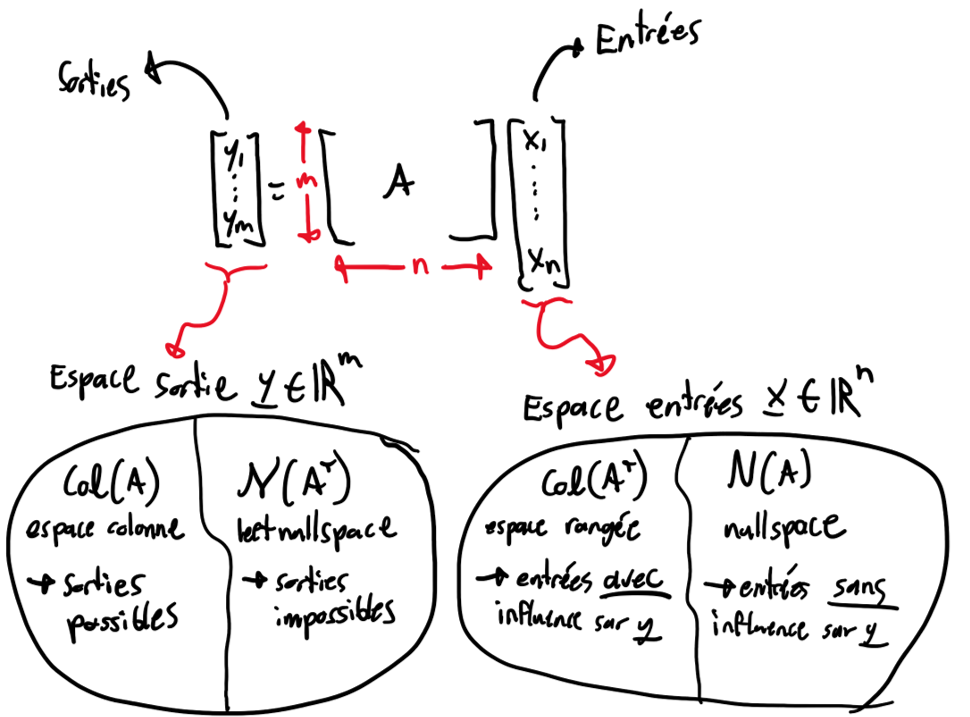
\includegraphics[width=0.80\textwidth]{linalgebra_4spaces.png}
	\caption{Quatres espaces fondamentaux d'une matrice}
	\label{fig:4spaces}
\end{figure}
%%%%%%%%%%%%%%%%%%%%%%%%%%%%%%%%%%%%%%%%%%%%%%%%%%%%%%%%%%%%%

%%%%%%%%%%%%%%%%%%%%%%%%%%%%%%%%%%%%%%%%%%%%%%%%%%%%%%%%%%%%
\begin{figure}[H]
	\centering
		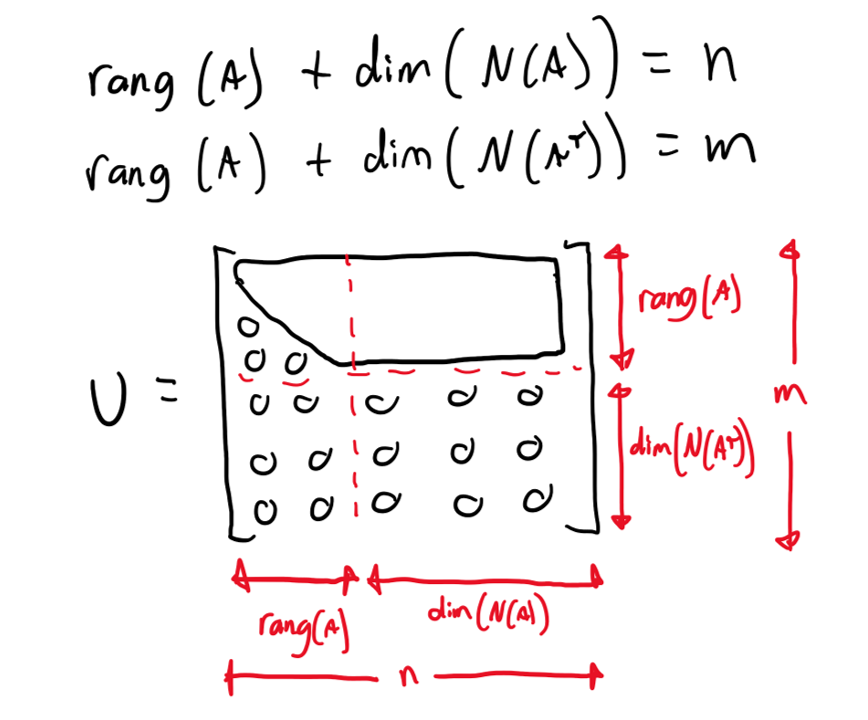
\includegraphics[width=0.60\textwidth]{linalgebra_4spaces2.png}
	\caption{Dimensions des quatre espaces fondamentaux d'une matrice}
	\label{fig:4spaces2}
\end{figure}
%%%%%%%%%%%%%%%%%%%%%%%%%%%%%%%%%%%%%%%%%%%%%%%%%%%%%%%%%%%%


%%%%%%%%%%%%%%%%%%%%%%%%%%%%%%%%%%%%%%%%%%%%%%%%%%%%%%%%%%
\subsection{Espace colonne}
\label{sec:espcol}
%%%%%%%%%%%%%%%%%%%%%%%%%%%%%%%%%%%%%%%%%%%%%%%%%%%%%%%%%%

L'espace colonne d'une matrice $A$ représente l'ensemble de toutes les valeurs possible de la sortie $\col{y}$ qui résulte de l'opération $\col{y} = A \col{x}$. Avec l'interprétation présentée à la section \ref{sec:combveccol}, il est possible de voir que la sortie $\col{y}$ a comme domaine toutes les combinaisons linéaires possibles des vecteur-colonnes de la matrice. Comme illustré à la Figure \ref{fig:2dspace}, pour une matrice qui aurait deux colonnes, si on interprète ces deux colonnes comme les composantes de vecteurs spatiaux, alors le domaine possible pour la sortie $\col{y}$ va être le plan formé par ces deux vecteurs.
%%%%%%%%%%%%%%%%%%%%%%%%%%%%%%%%%%%%%%%%%%%%%%%%%%%%%%%%%%%%%
\begin{figure}[H]
	\centering
		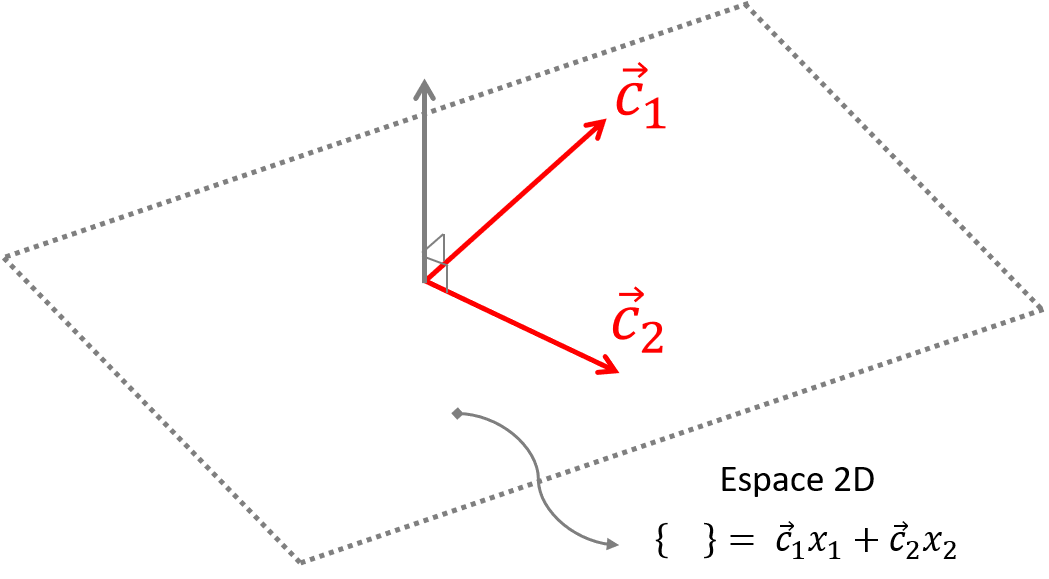
\includegraphics[width=0.60\textwidth]{2dspace.png}
	\caption{Visualisation graphique d'un espace colonne de dimension 2}
	\label{fig:2dspace}
\end{figure}
%%%%%%%%%%%%%%%%%%%%%%%%%%%%%%%%%%%%%%%%%%%%%%%%%%%%%%%%%%%%

L'espace colonne d'une matrice $A$ sera noté $col(A)$ et a la définition mathématique suivante:
%%%%%%%%%%%%%%%%%%%%%
\begin{align}
col(A) = 
\{ A \col{x} \; | \; \col{x} \in \re^n \}
\label{eq:cola}
\end{align}
%%%%%%%%%%%%%%%%%%%%%%

\note{Notation mathématique pour les ensembles:}{ Les crochets $\{ \}$ représentent un ensemble, à l'intérieur on note la liste des éléments de l'ensemble ou bien la définition. La barre verticale $|$ signifie \textit{tel que} et le symbole $\in$ signifie \textit{appartient à}. L'équation \eqref{eq:cola} peut donc se lire \textit{l'espace colonne de la matrice $A$ est égale à l'ensemble des résultats possible de l'opération $A \col{x} $ tel que $\col{x}$ appartient à l'espace vectoriel de dimension $n$}.}

Lorsque la matrice $A$ est inversible, i.e. de rang plein, l'espace colonne correspond à $\re^m$, ou $m$ est le nombre de variables de sortie. Par exemple, pour une matrice 3$\times$3 avec une sortie $\col{y}$ qui représente une position spatiale (x,y,z), si les colonnes ne sont pas co-planaire, alors la sortie $\col{y}$ va être une valeur arbitraire en 3D. On va donc dire que la matrice est inversible, car ici il est toujours possible de trouver une combinaison des colonnes pour obtenir un point (x,y,z) arbitraire. Toutefois, si les vecteurs-colonnes de la matrice sont co-linéaire (donc  ils forment un plan), alors l'espace colonne est restreint à ce plan. La sortie $\col{y}$ peut seulement prendre des valeurs qui correspondent à ce plan. Dans cette situation la matrice est dite non-inversible.


%%%%%%%%%%%%%%%%%%%%%%%%%%%%%%%%%%%%%%%%%%%%%%%%%%%%%%%%%%
\subsection{Espace nul gauche}
\label{sec:leftnullspace}
%%%%%%%%%%%%%%%%%%%%%%%%%%%%%%%%%%%%%%%%%%%%%%%%%%%%%%%%%%

L'espace nul gauche (\textit{Left-Nullspace}) d'une matrice $A$, noté $N(A^T)$, correspond au domaine de la sortie $\col{y}$ qui n'est pas dans l'espace colonne. Ce domaine correspond donc aux vecteurs $\col{y}$ qui sont impossible à obtenir peut importe le vecteur d'entrée $\col{x}$. L'espace nul gauche correspond aussi à l'ensemble de tous les vecteur-colonnes $\col{y}$ pour lesquels la multiplication avec la matrice $A^T$ donne un vecteur-colonne nulle $\col{0}$ :
%%%%%%%%%%%%%%%%%%%%%%%%%%%
\begin{align}
N(A^T) = \left\{ \col{y} \in \mathbb{R}^m \,|\, A^T\col{y} = \col{0} \right\}
\end{align}
%%%%%%%%%%%%%%%%%%%%%%%%%%%
une condition qui revient à dire que c'est l'espace nul gauche correspond à l'ensemble des vecteurs $\col{y}$ qui sont perpendiculaires à toutes les colonnes de la matrice $A$.


L'espace des vecteur-colonnes sorties $\col{y}$ est formé par $r$ (rang) bases qui forment l'espace colonne et $m-r$ bases qui forment l'espace nul gauche.
%%%%%%%%%%%%%%%%%%%%%%%%%%%
\begin{align}
m     = dim( col(A) ) + dim( N(A^T) )  = r + dim( N(A^T) )
\end{align}
%%%%%%%%%%%%%%%%%%%%%%%%%%%
%TODO Ajuster cela!!
% Tous les vecteur-colonnes sorties $\col{y}$ appartiennent soit à l'espace colonne soit à espace nul gauche:
% %%%%%%%%%%%%%%%%%%%%%%%%%%%
% \begin{align}
% \col{y} \in \re^m = col(A) \; \cup \; N(A^T) %\quad \text{et} \quad
% %n     = dim( row(A) ) + dim( N(A) ) 
% \end{align}
% %%%%%%%%%%%%%%%%%%%%%%%%%%%
%
\textbf{Les vecteur-colonnes $\col{y}$ appartenant à l'espace colonne ont une solution $\col{x}$ possible, tandis que ceux appartenant à l'espace nul gauche n'ont aucune solution exacte $\col{x}$ possible}.
%
Une matrice $A$ va avoir un espace nul gauche seulement lorsqu'elle a une rang déficient. La présence d'un espace nul gauche indique un système sur-contraint, i.e. un surplus d'équations. Il y aura donc plusieurs sorties $\col{y}$ pour lesquelles il n'y a pas de solutions $\col{x}$.


\begin{example}[Espace-nul gauche de la matrice jacobienne d'un robot manipulateur]
%%%%%%%%%%%%%%%%%%%%%%%%%%%%%%%%%%%%%%%%%%%%%%%%%%%%%%%%%%%%
\begin{figure}[H]
	\centering
		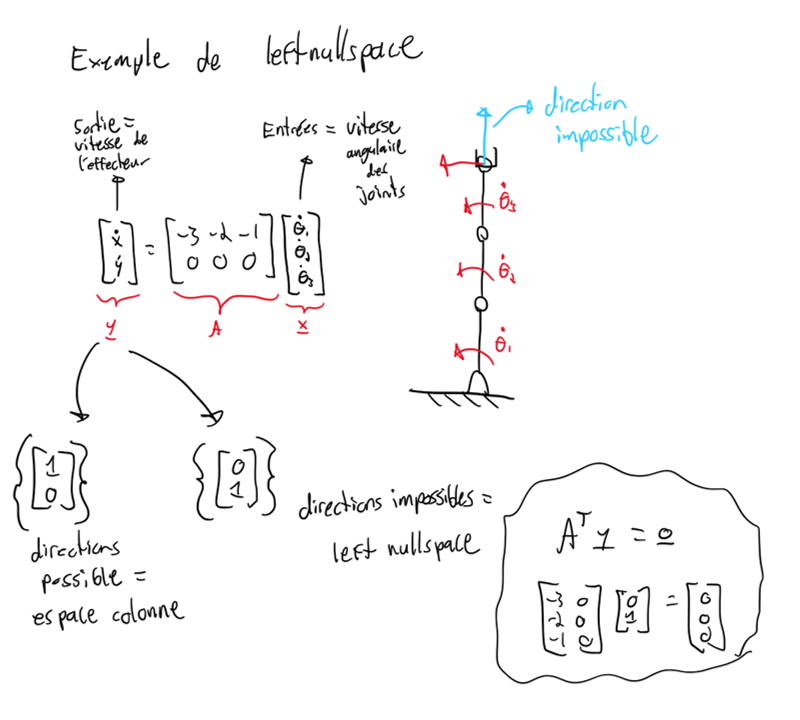
\includegraphics[width=0.80\textwidth]{linalgebra_4spaces_ex2.png}
	\caption{Exemple de l'espace-nul gauche d'une matrice}
	\label{fig:4spaces_ex2}
\end{figure}
%%%%%%%%%%%%%%%%%%%%%%%%%%%%%%%%%%%%%%%%%%%%%%%%%%%%%%%%%%%%
\end{example}



%%%%%%%%%%%%%%%%%%%%%%%%%%%%%%%%%%%%%%%%%%%%%%%%%%%%%%%%%%
\subsection{Espace nul}
\label{sec:nullspace}
%%%%%%%%%%%%%%%%%%%%%%%%%%%%%%%%%%%%%%%%%%%%%%%%%%%%%%%%%%

L'espace nul (\textit{Nullspace}) d'une matrice $A$, noté $N(A)$ correspond a l'ensemble de tous les vecteur-colonnes $\col{x}$ pour lesquels la multiplication avec la matrice $A$ donne un vecteur-colonne nulle $\col{0}$ :
%%%%%%%%%%%%%%%%%%%%%%%%%%%
\begin{align}
N(A) = \left\{ \col{x} \in \mathbb{R}^n \,|\, A\col{x} = \col{0} \right\}
\end{align}
%%%%%%%%%%%%%%%%%%%%%%%%%%%

Une matrice $A$ va avoir un espace nul seulement lorsqu'elle a une rang déficient, donc des colonnes linéairement dépendantes. La présence d'un espace nul indique un système sous-contraint ou il y a un surplus de variables, donc plusieurs solutions possibles d'entrées $\col{x}$ pour obtenir une même sortie $\col{y}$. 
%
%\textbf{Utilisation} Une utilité du \textit{Nullspace} est que si on connaît un solution $\col{x}_s$ tel que: 
%%%%%%%%%%%%%%%%%%%%%%%%%%%%
%\begin{align}
%A \col{x}_s = \col{y}
%\end{align}
%%%%%%%%%%%%%%%%%%%%%%%%%%%%
%Il est possible de trouver les autres solutions possible directement si on connaît le \textit{Nullspace}, car une addition de la solution connue et d'un vecteur-colonne appartenant au \textit{Nullspace} ($\col{x}_n \in N(A) $)  est aussi une solution: 
%%%%%%%%%%%%%%%%%%%%%%%%%%%%
%\begin{align}
%A ( \col{x}_s + \col{x}_n) = A \col{x}_s + 
%\underbrace{
%A \col{x}_n 
%}_{ \col{0} }
%= A \col{x}_s = \col{y}
%\end{align}
%%%%%%%%%%%%%%%%%%%%%%%%%%%%
%

\newpage
\begin{example}[Espace-nul de la matrice jacobienne d'un robot manipulateur]
La figure \ref{fig:4spaces_ex1} illustre la signification physique de l'espace nul d'une matrice qui relie la vitesse des joints d'un robot manipulateur à la vitesse de son effecteur.
%%%%%%%%%%%%%%%%%%%%%%%%%%%%%%%%%%%%%%%%%%%%%%%%%%%%%%%%%%%%
\begin{figure}[H]
	\centering
		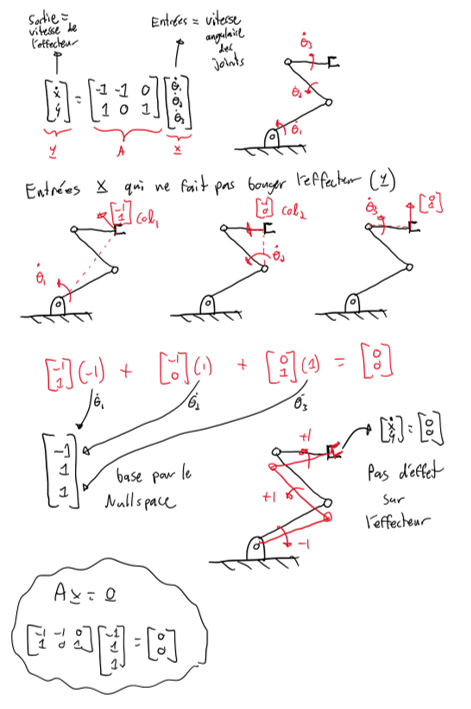
\includegraphics[width=0.80\textwidth]{linalgebra_4spaces_ex1.png}
	\caption{Exemple de l'espace nul d'une matrice}
	\label{fig:4spaces_ex1}
\end{figure}
%%%%%%%%%%%%%%%%%%%%%%%%%%%%%%%%%%%%%%%%%%%%%%%%%%%%%%%%%%%%
\end{example}


%%%%%%%%%%%%%%%%%%%%%%%%%%%%%%%%%%%%%%%%%%%%%%%%%%%%%%%%%%
\subsection{Espace rangée}
\label{sec:esprow}
%%%%%%%%%%%%%%%%%%%%%%%%%%%%%%%%%%%%%%%%%%%%%%%%%%%%%%%%%%

%L'espace rangé d'une matrice correspond à l'ensemble des vecteur-colonnes entrées $\col{x}$ qui donnent un vecteur-colonne sortie $\col{y}$ non-nul lorsque multiplié par la matrice $A$.
L'espace rangé correspond à toutes les combinaisons possibles des rangées de la matrice $A$, ce qui est donc équivalent à toutes les combinaisons possibles des colonnes de la matrice transposée $A^T$. L'espace rangée d'une matrice $A$ sera noté $row(A)$ et a la définition suivante:
%%%%%%%%%%%%%%%%%%%
\begin{align}
row(A) =  col(A^T) = 
\{ A^T \col{y} \; | \; \col{y} \in \re^m \}
\end{align}
%%%%%%%%%%%%%%%%%%%
Lorsque la matrice $A$ est inversible, i.e. de rang plein, l'espace rangé correspond à $\re^n$, ou $n$ est le nombre de variables d'entrées.


L'espace des vecteur-colonnes entrées $\col{x}$ est formé par $r$ (rang) bases qui forment l'espace rangée et $n-r$ bases qui forment l'espace nul:
%%%%%%%%%%%%%%%%%%%%%%%%%%%
\begin{align}
n     = dim( row(A) ) + dim( N(A) )  = r + dim( N(A) )
\end{align}
%%%%%%%%%%%%%%%%%%%%%%%%%%%
%TODO Ajuster cela!!
% Tous les vecteur-colonnes entrées $\col{x}$ pour une matrice appartiennent soit à l'espace rangé soit à l'espace nul:
% %%%%%%%%%%%%%%%%%%%%%%%%%%%
% \begin{align}
% \col{x} \in \re^n = col(A^T) \; \cup \; N(A) %\quad \text{et} \quad
% %n     = dim( row(A) ) + dim( N(A) ) 
% \end{align}
% %%%%%%%%%%%%%%%%%%%%%%%%%%%

\textbf{Les vecteur-colonnes appartenant à l'espace rangé influencent la sortie alors que les vecteur-colonnes appartenant à l'espace nul n'influent pas la sortie.} 






%%%%%%%%%%%%%%%%%%%%%%%%%%%%%%%%%%%%%%%%%%%%%%%%%%%%%%%%%%
\subsection{Rang d'une matrice}
\label{sec:rang}
%%%%%%%%%%%%%%%%%%%%%%%%%%%%%%%%%%%%%%%%%%%%%%%%%%%%%%%%%%

Le rang $r$ d'une matrice correspond à la dimension de l'espace colonne d'une matrice, qui est toujours aussi égale à la dimension de l'espace rangé. Ce nombre correspond aussi au nombre de pivots, il sera noté par la variable $r$:
%%%%%%%%%%%%%%%%%%%%%%
\begin{align}
r = rank( A ) = dim( col(A) ) = dim( col(A^T) ) =\#\, pivots
\end{align}
%%%%%%%%%%%%%%%%%%%%%%%

Le rang d'une matrice est toujours inférieur ou égale aux dimensions $m$ et $n$.
%%%%%%%%%%%%%%%%%%%%%%%
\begin{align}
r \leq n &= \#\, ranges \\
r \leq m &= \#\, colonnes
\end{align}
%%%%%%%%%%%%%%%%%%%%%%%%

Dans le cas d'une matrice carré ($m=n$), il est possible de déterminer si la matrice à une rang dit plein, i.e. si $r=m=n$, en calculant le déterminant de la matrice $A$. Si le déterminant est non-nul alors la matrice à un rang plein.  


\newpage
%%%%%%%%%%%%%%%%%%%%%%%%%%%%%%%%%%%%%%%%%%%%%%%%%%%%%%%%%%
\subsection{Quatre situations possibles pour un système d'équations}
\label{sec:rangpleinvstrop}
%%%%%%%%%%%%%%%%%%%%%%%%%%%%%%%%%%%%%%%%%%%%%%%%%%%%%%%%%%

Un système d'équations peut être parfaitement contraint (une seule solution existe), sur-contraint (aucune solution exacte n'existe) ou bien sous-contraint (plusieurs solutions sont possible. Dans le cas d'une relation matricielle de type $A \col{x} = \col{y} $, qui représente un système d’équations linéaires, le rang de la matrice $A$ permet de déterminer la situation, voir figure \ref{fig:rmn}.

%%%%%%%%%%%%%%%%%%%%%%%%%%%%%%%%%%%%%%%%%%%%%%%%%%%%%%%%%%%%%
\begin{figure}[htp]
	\centering
		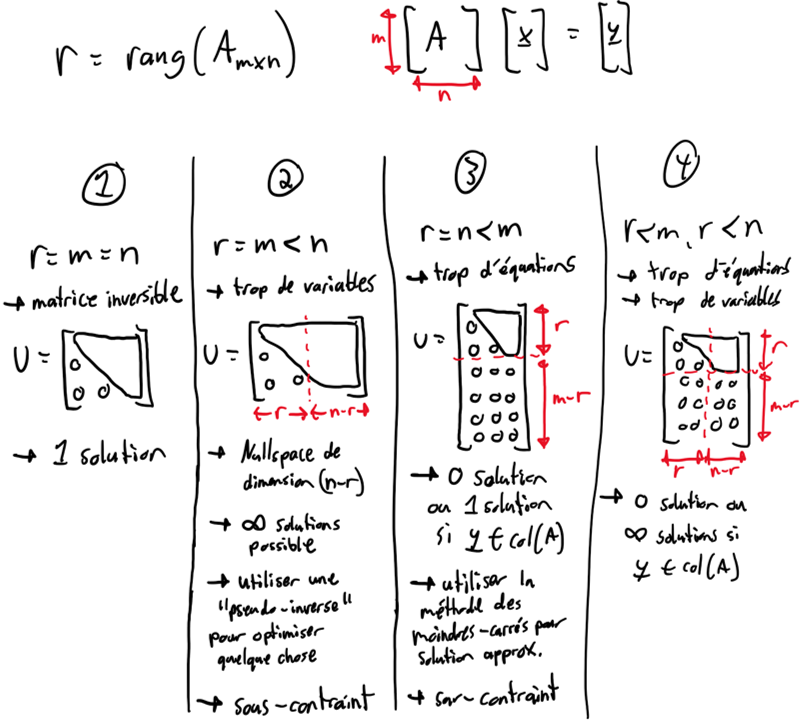
\includegraphics[width=0.95\textwidth]{linalgebra_4types.png}
	\caption{Quatre situations possibles pour un système d'équations}
	\label{fig:rmn}
\end{figure}
%%%%%%%%%%%%%%%%%%%%%%%%%%%%%%%%%%%%%%%%%%%%%%%%%%%%%%%%%%%%

Les grandes catégories de situations possibles illustrés à la figure \ref{fig:rmn} sont exemplifiés avec les exemples illustrés aux figures \ref{fig:rmn_ex1}, \ref{fig:rmn_ex2}, \ref{fig:rmn_ex3} et \ref{fig:rmn_ex4}.

\begin{enumerate}
    \item Parfaitement contraint ($r=m=n$): Il n'y a pas d'espace nul ni d'espace gauche nul.
    \item Trop de variables ($r<n$): Il y a un espace nul de dimension $n-r$.
    \item Trop d'équations ($r<m$): Il y a un espace gauche nul de dimension $m-r$.
    \item Trop d'équations et de variables ($r<m,r<n$): Il y a un espace gauche nul de dimension $m-r$ et un espace nul de dimension $n-r$.
\end{enumerate}




\newpage
\begin{example}[Système d'équation parfaitement contraint]
%%%%%%%%%%%%%%%%%%%%%%%%%%%%%%%%%%%%%%%%%%%%%%%%%%%%%%%%%%%%%
\begin{figure}[H]
	\centering
		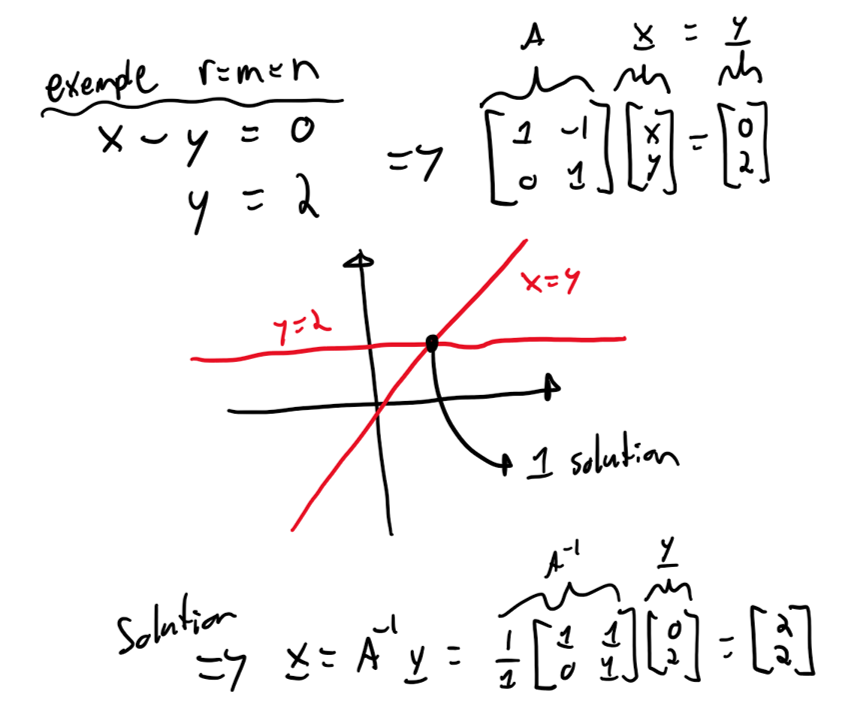
\includegraphics[width=0.60\textwidth]{linalgebra_4types_ex1.png}
	\caption{Exemple d'un système d'équation parfaitement contraint}
	\label{fig:rmn_ex1}
\end{figure}
%%%%%%%%%%%%%%%%%%%%%%%%%%%%%%%%%%%%%%%%%%%%%%%%%%%%%%%%%%%%
\end{example}

\begin{example}[Système d'équation sous-contraint]
%%%%%%%%%%%%%%%%%%%%%%%%%%%%%%%%%%%%%%%%%%%%%%%%%%%%%%%%%%%
\begin{figure}[H]
	\centering
		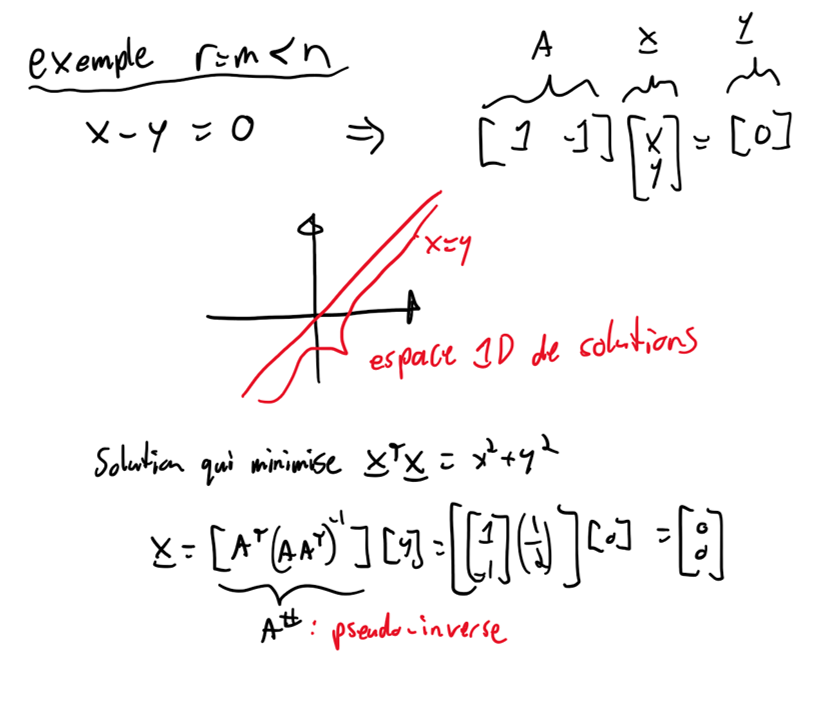
\includegraphics[width=0.60\textwidth]{linalgebra_4types_ex2.png}
	\caption{Exemple d'un système d'équation sous-contraint}
	\label{fig:rmn_ex2}
\end{figure}
%%%%%%%%%%%%%%%%%%%%%%%%%%%%%%%%%%%%%%%%%%%%%%%%%%%%%%%%%%%%
\end{example}

\begin{example}[Système d'équation sur-contraint]
%%%%%%%%%%%%%%%%%%%%%%%%%%%%%%%%%%%%%%%%%%%%%%%%%%%%%%%%%%%%
\begin{figure}[H]
	\centering
		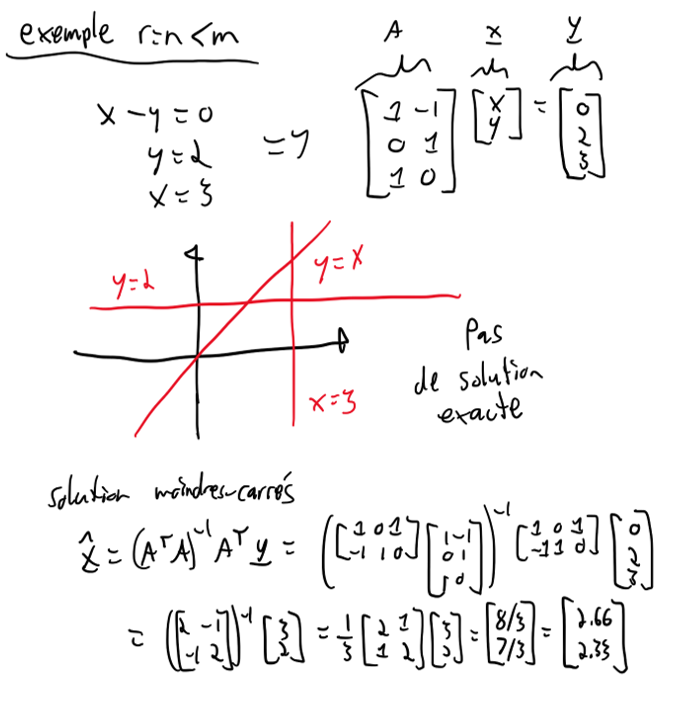
\includegraphics[width=0.50\textwidth]{linalgebra_4types_ex3.png}
	\caption{Exemple d'un système d'équation sur-contraint}
	\label{fig:rmn_ex3}
\end{figure}
%%%%%%%%%%%%%%%%%%%%%%%%%%%%%%%%%%%%%%%%%%%%%%%%%%%%%%%%%%%%%
\end{example}

\begin{example}[Système d'équation non-inversible]
%%%%%%%%%%%%%%%%%%%%%%%%%%%%%%%%%%%%%%%%%%%%%%%%%%%%%%%%%%%%%
\begin{figure}[H]
	\centering
		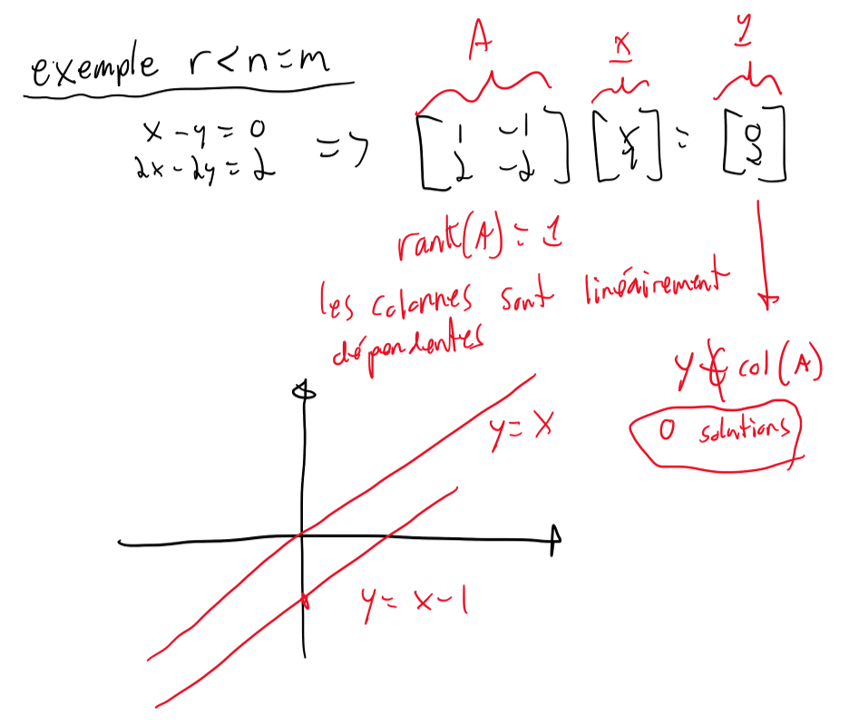
\includegraphics[width=0.50\textwidth]{linalgebra_4types_ex4.png}
	\caption{Exemple d'un système d'équation non-inversible}
	\label{fig:rmn_ex4}
\end{figure}
%%%%%%%%%%%%%%%%%%%%%%%%%%%%%%%%%%%%%%%%%%%%%%%%%%%%%%%%%%%%%
\end{example}


%%%%%%%%%%%%%%%%%%%%%%%%%%%%%%%%%%%%%%%%%%%%%%%%%%%%%%%%%%
\subsection{Factorisation LU}
\label{sec:lu}
%%%%%%%%%%%%%%%%%%%%%%%%%%%%%%%%%%%%%%%%%%%%%%%%%%%%%%%%%%

Une matrice $A$ peut-être factorisée en deux matrices (triangulaires lorsque $A$ est une matrice inversible):
%
\begin{align}
A = LU 
\end{align}
%
où la matrice $U$ est une matrice ou tout les coefficients sous la diagonale sont nuls et la matrice $L$ correspond aux opérations sur les ranges conduites dans le cadre d'une élimination Gauss-Jordan. Par exemple pour une matrice 3x3 inversible:
%
\begin{align}
L= 
\left[ \begin{array}{c c c } 
1      &   0       & 0   \\ 
l_{21} &   1       & 0   \\  
l_{31} & l_{32}    & 1
\end{array} \right]
\quad\quad
U = 
\left[ \begin{array}{c c c c c } 
p_{1} & u_{12} &  u_{13} \\ 
0     & p_{2}  &  u_{23}  \\ 
0     & 0      &  p_{3}
\end{array} \right]
\end{align}
%
Les coefficients non-nuls $p_i$ sur la diagonale de la matrice $U$ sont appeles les pivots.



%%%%%%%%%%%%%%%%%%%%%%%%%%%%%%%%%%%%%%%%%%%%%%%%%%%%%%%%%%
\subsection{Base}
\label{sec:base}
%%%%%%%%%%%%%%%%%%%%%%%%%%%%%%%%%%%%%%%%%%%%%%%%%%%%%%%%%%

Un ensemble $\{ \col{v}_1 \; \col{v}_2 \; \hdots \; \col{v}_n \}$ de vecteurs de dimensions $m$ dans un espace vectoriel appartenant à $\re^m$, forme une base de cet espace si: \textbf{1)} les vecteurs $\col{v}_1 \; \col{v}_2 \; \hdots \; \col{v}_n$ sont linéairement indépendants et \textbf{2)} tout vecteur $\col{w}$ de cet espace peut être exprimé comme une combinaison linéaire de ces vecteurs:
%%%%%%%%%%%%%%%%%%%%%%
\begin{align}
\col{w} = x_1 \col{v}_1 + x_2 \col{v}_2 + ... + x_n \col{v}_n
\end{align}
%%%%%%%%%%%%%%%%%%%%%%%

Par exemple, dans un espace tri-dimensionnel qui correspond à des coordonnées $
\left[
\begin{array}{c}
x \\ y \\ z
\end{array}
\right]
$, les vecteur-colonnes $\left\{ 
\left[
\begin{array}{c}
1 \\ 0 \\ 0
\end{array}
\right],
\left[
\begin{array}{c}
0 \\ 1 \\ 0
\end{array}
\right]
\right\}$
forment une base pour le sous-espace qui correspond au plan $z=0$.

%%%%%%%%%%%%%%%%%%%%%%%%%%%%%%%%%%%%%%%%%%%%%%%%%%%%%%%%%%
\subsection{Indépendance linéaire}
\label{sec:lindep}
%%%%%%%%%%%%%%%%%%%%%%%%%%%%%%%%%%%%%%%%%%%%%%%%%%%%%%%%%%

Un vecteur est dit linéairement dépendant d'un autre vecteur (ou un ensemble de vecteurs), lorsque celui-ci peut être exprimé comme une combinaison pondéré des autres. 

%TODO figure

Un ensemble de vecteurs $\left\{ \col{v}_1, \col{v}_2, \hdots, \col{v}_n \right\}$ est \textbf{linéairement dépendant} s'il existe des coefficients non nuls $x_i$ tels que la somme pondérée des vecteurs est nulle:
%%%%%%%%%%%%%%%%%%%%%%
\begin{align}
\col{0} = x_1 \col{v}_1 + x_2 \col{v}_2 + ... + x_n \col{v}_n
\end{align}
%%%%%%%%%%%%%%%%%%%%%%%

Inversement, un ensemble de vecteurs $\left\{ \col{v}_1, \col{v}_2, \hdots, \col{v}_n \right\}$ est \textbf{linéairement indépendant} si:
%%%%%%%%%%%%%%%%%%%%%%
\begin{align}
\col{0} = x_1 \col{v}_1 + x_2 \col{v}_2 + ... + x_n \col{v}_n
\quad
\text{implique que:}
\quad
0 = x_1 = x_2 = ... = x_n 
\end{align}
%%%%%%%%%%%%%%%%%%%%%%%




% %%%%%%%%%%%%%%%%%%%%%%%%%%%%%%%%%%%%%%%%%%%%%%%%%%%%%%%%%%%%
% \section{Projection}
% \label{sec:projectionmatrix}
% %%%%%%%%%%%%%%%%%%%%%%%%%%%%%%%%%%%%%%%%%%%%%%%%%%%%%%%%%%%%

% À venir!

\newpage
%%%%%%%%%%%%%%%%%%%%%%%%%%%%%%%%%%%%%%%%%%%%%%%%%%%%%%%%%%%%
\section{Moindres carrés}
\label{sec:moindrecarre}
%%%%%%%%%%%%%%%%%%%%%%%%%%%%%%%%%%%%%%%%%%%%%%%%%%%%%%%%%%%%

Lorsqu'un système d'équation linéaire $\col{y} = A \col{x}$ est sur-contraint, c'est-à-dire que le vecteur $\col{y}$ n'est pas dans l'espace colonne de la matrice $A$, il n'y a pas de solution exacte possible. Il est toutefois possible de calculer une solution approximée qui minimise la norme de l'erreur avec une expression explicite:
%%%%%%%%%%%%%%%%%%%%%%%%%%%
\begin{align}
\col{\hat{x}}^* &= \operatornamewithlimits{argmin}\limits_{\col{\hat{x}}} \left\| A \col{\hat{x}} - \col{y} \right\|^2
= (A^T A)^{-1} A^T \, \col{y}
\end{align}
%%%%%%%%%%%%%%%%%%%%%%%%%%%
%%%%%%%%%%%%%%%%%%%%%%%%%%%%%%%%%%%%%%%%%%%%%%%%%%%%%%%%%%%%
\begin{figure}[htbp]
	\centering
		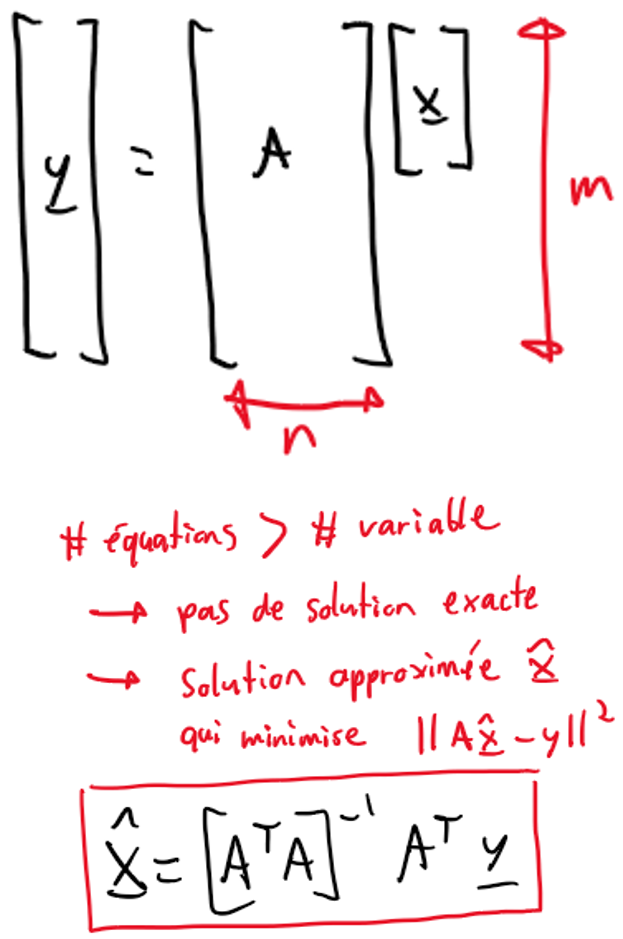
\includegraphics[width=0.5\textwidth]{leastsquare.png}
	\caption{Système sur-contraint: solution des moindres-carrés}
	\label{fig:leastsquare}
\end{figure}
%%%%%%%%%%%%%%%%%%%%%%%%%%%%%%%%%%%%%%%%%%%%%%%%%%%%%%%%%%%%

La matrice $(A^T A)^{-1} A^T$ est souvent appelée inverse gauche de Moore–Penrose et notée:
%%%%%%%%%%%%%%%%%%%%%%%%%%%
\begin{align}
A^{+} &= (A^T A)^{-1} A^T  \quad \Rightarrow \quad A^{+} A = I
\end{align}
%%%%%%%%%%%%%%%%%%%%%%%%%%%

Il est à noter que la matrice $A$ doit avoir des colonnes indépendantes pour que la matrice $A^T A$ soit inversible et donc pour que la méthode des moindres-carrés fonctionne.


\subsection{Application à des problèmes d'identification de paramètres}


La méthode des moindres-carrés est très utile pour identifier des paramètres inconnus dans une relation linéaire. Lorsqu'on a un modèle linéaire qui implique des signaux connus et des paramètres inconnus qui peut être exprimé sous la forme:
%%%%%%%%%%%%%%%%%%%%%%%%%%%%%%%%%%%%%%%%%%%%%%
\begin{align}
\underline{\varphi}^T \underline{\theta}
= b
\quad\quad\Rightarrow\quad\quad
\underbrace{ 
\left[ \begin{array}{c c c } 
\varphi_1 & ... & \varphi_m
\end{array} \right] }_{ m \text{ signaux connus} }
\underbrace{ \left[ \begin{array}{c} 
\theta_1 \\ \vdots \\ \theta_m
\end{array} \right] }_{ m \text{ paramètre inconnus} } = 
\underbrace{b}_{\text{signal connu} }
\end{align}
%%%%%%%%%%%%%%%%%%%%%%%%%%%%%%%%%%%%%%%%%%%%%
Il est possible de regrouper plusieurs mesures expérimentales dans un système matricielle:
%%%%%%%%%%%%%%%%%%%%%%%%%%%%%%%%%%%%%%%%%%%%%
\begin{align}
A \underline{\theta}
= \underline{b}
\quad\quad\Rightarrow\quad\quad
\underbrace{ 
\left[ \begin{array}{c c c c c } 
&& \underline{\varphi}^T(1) && \\
&& \vdots & \\
&& \underline{\varphi}^T(N) && \\
\end{array} \right] }_{\text{ $A$ : $N \times m$  known samples} }
\left[ \begin{array}{c} 
\theta_1 \\ \vdots \\ \theta_m
\end{array} \right]
 = \underbrace{ \left[ \begin{array}{c}  
b(1) \\ \vdots \\ b(N)\\ 
 \end{array} \right] }_{ \text{ $\underline{b}$: $N$ known samples} } 
\end{align}
%%%%%%%%%%%%%%%%%%%%%%%%%%%%%%%%%%%%%%%%%%%%%
Pour ensuite utiliser la méthode des moindres-carrés pour obtenir un estimé des paramètres inconnus qui minimise l'erreur avec les mesures expérimentales:
%%%%%%%%%%%%%%%%%%%%%%%%%%%
\begin{align}
\col{\hat{\theta}}^* &= \operatornamewithlimits{argmin}\limits_{\col{\hat{\theta}}} \left\| A \col{\hat{\theta}} - \col{b} \right\|^2
= (A^T A)^{-1} A^T \, \col{b}
\end{align}
%%%%%%%%%%%%%%%%%%%%%%%%%%%



\begin{example}[Régression linéaire avec les moindres-carrés]
%%%%%%%%%%%%%%%%%%%%%%%%%%%%%%%%%%%%%%%%%%%%%%%%%%%%%%%%%%%%
\begin{figure}[H]
	\centering
		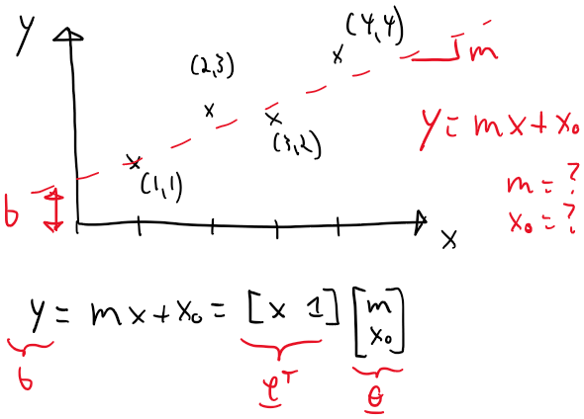
\includegraphics[width=0.5\textwidth]{regression_ex1.png}
		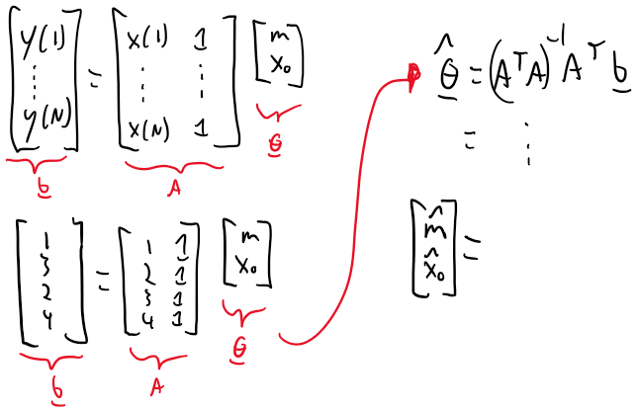
\includegraphics[width=0.5\textwidth]{regression_ex2.png}
	\caption{Régression linéaire avec les moindres-carrés pour identifier les paramètres d'une ligne}
	\label{fig:regression-ex1}
\end{figure}
%%%%%%%%%%%%%%%%%%%%%%%%%%%%%%%%%%%%%%%%%%%%%%%%%%%%%%%%%%%%
\end{example}

\begin{proof}
La solution des moindres-carrés minimise une fonction coût qui est défini comme le carré de la norme du vecteur d'erreur, qui correspond à la somme des carrés des erreurs individuelles pour chaque sortie du système:
%%%%%%%%%%%%%%%%%%%%%%%%%%%
\begin{align}
J = \left\| \col{e} \right\|^2  = \col{e}^T\col{e} = \sum{ e_i^2}
\end{align}
%%%%%%%%%%%%%%%%%%%%%%%%%%%
L'erreur est définie comme la différence entre les sorties $\col{y}$ et le résultat du calcul $A \col{\hat{x}}$:
%%%%%%%%%%%%%%%%%%%%%%%%%%%
\begin{align}
\col{e} = A \col{\hat{x}} - \col{y}
\end{align}
%%%%%%%%%%%%%%%%%%%%%%%%%%%
Il est ensuite possible de trouver le minimum de la fonction coût $J$ en trouvant le point pour lequel toutes les dérivées par rapport à $\col{\hat{x}}$ sont nulles:
%%%%%%%%%%%%%%%%%%%%%%%%%%%
\begin{align}
\col{0} &= \frac{\partial J}{\partial \col{\hat{x}}} \\
\col{0} &= \frac{\partial \col{e}^T\col{e}}{\partial \col{\hat{x}}} \\
\col{0} &= 2 \col{e}^T \frac{\partial e }{\partial \col{\hat{x}}} \\
\col{0} &= 2 ( A \col{\hat{x}} -\col{y} )^T \frac{\partial (A \col{\hat{x}} -\col{y}) }{\partial \col{\hat{x}}} \\
\col{0} &= 2 ( A \col{\hat{x}} -\col{y}  )^T A  \\
\col{0} &=  \col{\hat{x}}^T A^T A  - \col{y}^T A   \\
A^T \col{y} &= A^T A \col{\hat{x}} \\
(A^T A)^{-1} A^T \col{y} &= \col{\hat{x}} 
\end{align}
%%%%%%%%%%%%%%%%%%%%%%%%%%%
\end{proof}


\iftoggle{EN}{%
%%%%%%%%%%%%%%%%%%%%%%%%%%%%%%%%%%%%%%%%%%%%%%%%%%%%%%%%%%%%%
\newpage
\subsection{Graphical Interpretation of the Least Square Solution}

Given an input-output model with linearly involved parameters:
\begin{align}
\underline{\varphi}^T \underline{\theta}
= y
\quad\quad\Rightarrow\quad\quad
\underbrace{ 
\left[ \begin{array}{c c c } 
\varphi_1 & ... & \varphi_m
\end{array} \right] }_{ m \text{ known inputs} }
\underbrace{ \left[ \begin{array}{c} 
\theta_1 \\ \vdots \\ \theta_m
\end{array} \right] }_{ m \text{ unknown parameters} } = 
\underbrace{y}_{\text{known scalar output} }
\end{align}

Given an $N$ samples of input-output data:
\begin{align}
\Phi^T \underline{\theta}
= \underline{y}
\quad\quad\Rightarrow\quad\quad
\underbrace{ 
\left[ \begin{array}{c c c c c } 
&& \underline{\varphi}^T(1) && \\
&& \vdots & \\
&& \underline{\varphi}^T(N) && \\
\end{array} \right] }_{\text{ $\Phi^T$ : $N \times m$  inputs data} }
\left[ \begin{array}{c} 
\theta_1 \\ \vdots \\ \theta_m
\end{array} \right]
 = \underbrace{ \left[ \begin{array}{c}  
 y(1) \\ \vdots \\ y(N)\\ 
 \end{array} \right] }_{ \text{ $\underline{y}$: $N$ output samples} } 
\end{align}

Column of matrix $\Phi^T$ span a $N$ dimension hyperplane:
%%%%%%%%%%%%%%%%%%%%%%%%%%%%%%%%%%%%%%%%%%%%%%%%%%%%%%%
\begin{align}
\Phi^T = 
\left[ \begin{array}{c@{}c@{}c}  
\left[  \begin{array}{c}  \\ \underline{c_1} \\ \\ \end{array} \right] &  \ldots & \left[  \begin{array}{c} \\ \underline{c_m} \\ \\ \end{array} \right]
\end{array} \right]
\end{align}
%%%%%%%%%%%%%%%%%%%%%%%%%%%%%%%%%%%%%%%%%%%%%%%%%%%%%%%%%%

Exact solution does not exist when $\underline{y} \notin col( \Phi^T )$, instead we look for an approximation:
\begin{align}
\text{Projection Approximation : }
\Phi^T \hat{\underline{\theta}}= \underline{p}
\quad\quad\quad
\text{Error : }
\underline{e} = \underline{y} - \underline{p}
\end{align}
The distance between the approximation $\underline{p}$ and $\underline{y}$ is minimal when the error $\underline{e}$ is orthogonal to the column space hyperplane:
\begin{align}
\underline{c}_i^T \underline{e}= 0 \quad \forall \, i
\quad\Rightarrow\quad
\Phi \underline{e}= \underline{0}
\quad\Rightarrow\quad
\Phi ( \, \underline{y} - \Phi^T \hat{\underline{\theta}} \, )= \underline{0}
\quad\Rightarrow\quad
\hat{\underline{\theta}} = \left[ \Phi \Phi^T \right]^{-1} \Phi \underline{y}
\end{align}

\begin{figure}[htp]
	\centering
		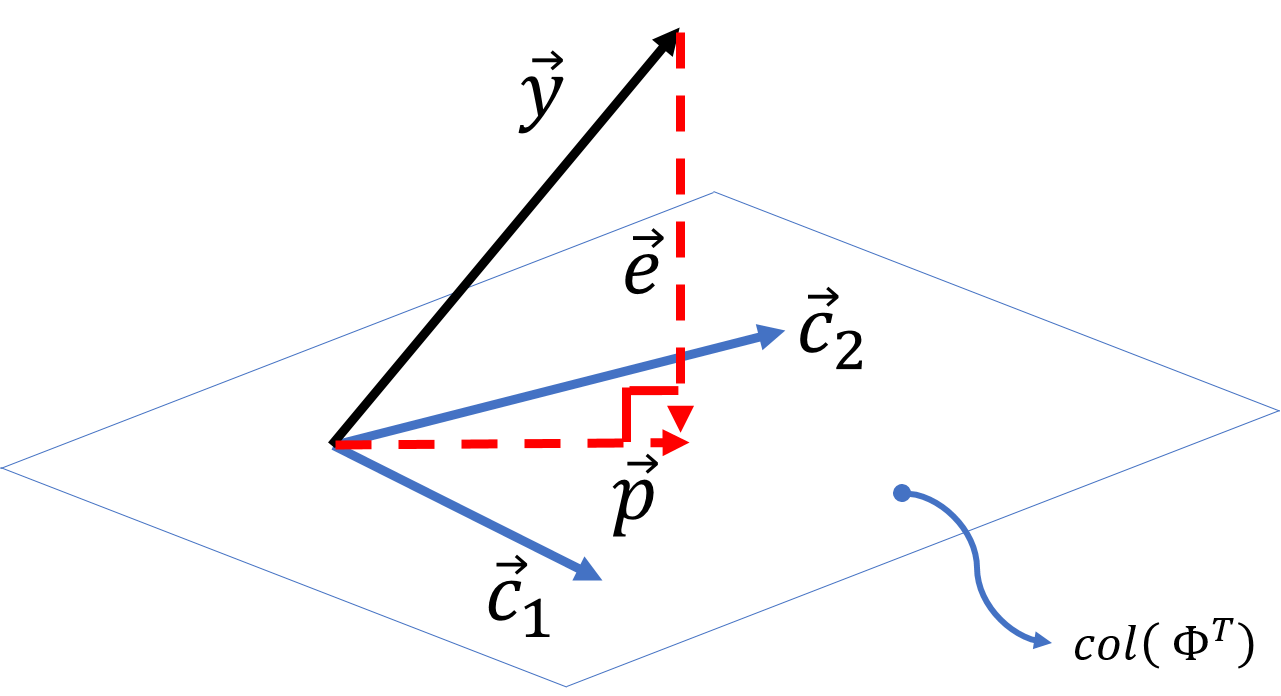
\includegraphics[width=0.45\textwidth]{projectionLS.png}
	\caption{Graphical Visualization of Least Square}
\end{figure}

}




\newpage
%%%%%%%%%%%%%%%%%%%%%%%%%%%%%%%%%%%%%%%%%%%%%%%%%%%%%%%%%%%%
\section{Pseudo-Inverse}
\label{sec:pseudoinverse}
%%%%%%%%%%%%%%%%%%%%%%%%%%%%%%%%%%%%%%%%%%%%%%%%%%%%%%%%%%%%

Lorsqu'un système d'équation linéaire $\col{y} = A \col{x}$ est sous-contraint, c'est-à-dire que plusieurs vecteurs $\col{x}$ sont des solutions, il est possible d'utiliser une matrice pseudo-inverse pour obtenir une solution qui optimise une fonction coût quadratique:
%%%%%%%%%%%%%%%%%%%%%%%%%%%
\begin{align}
\col{x}^* &= \operatornamewithlimits{argmin}\limits_{\col{x}} \left( \col{x}^T Q \col{x} \right) \quad \text{subject to} \quad \col{y} = A \col{x}  \\
\col{x}^* &= Q^{-1} A^T (A Q^{-1} A^T)^{-1} \, \col{y}
\end{align}
%%%%%%%%%%%%%%%%%%%%%%%%%%%
Dans un cas simplifié ou la matrice de poids $Q$ est réduite à une matrice identité on a:
%%%%%%%%%%%%%%%%%%%%%%%%%%%
\begin{align}
\col{x}^* &= \operatornamewithlimits{argmin}\limits_{\col{x}} \left\| \col{x} \right\|^2 \quad \text{subject to} \quad \col{y} = A \col{x}  \\
\col{x}^* &= A^T (A A^T)^{-1} \, \col{y}
\end{align}
%%%%%%%%%%%%%%%%%%%%%%%%%%%
La matrice $A^T (A A^T)^{-1}$ est souvent appelée inverse droit de Moore–Penrose et notée:
%%%%%%%%%%%%%%%%%%%%%%%%%%%
\begin{align}
A^{\#} &= A^T (A A^T)^{-1}  \quad \Rightarrow \quad A A^{\#} = I
\end{align}
%%%%%%%%%%%%%%%%%%%%%%%%%%%
Il est à noter que la matrice $A$ doit avoir des rangés indépendantes pour que la matrice $A A^T$ soit inversible et donc pour pouvoir utiliser la pseudo-inverse droite.

%%%%%%%%%%%%%%%%%%%%%%%%%%%%%%%%%%%%%%%%%%%%%%%%%%%%%%%%%%%%
\begin{figure}[htbp]
	\centering
		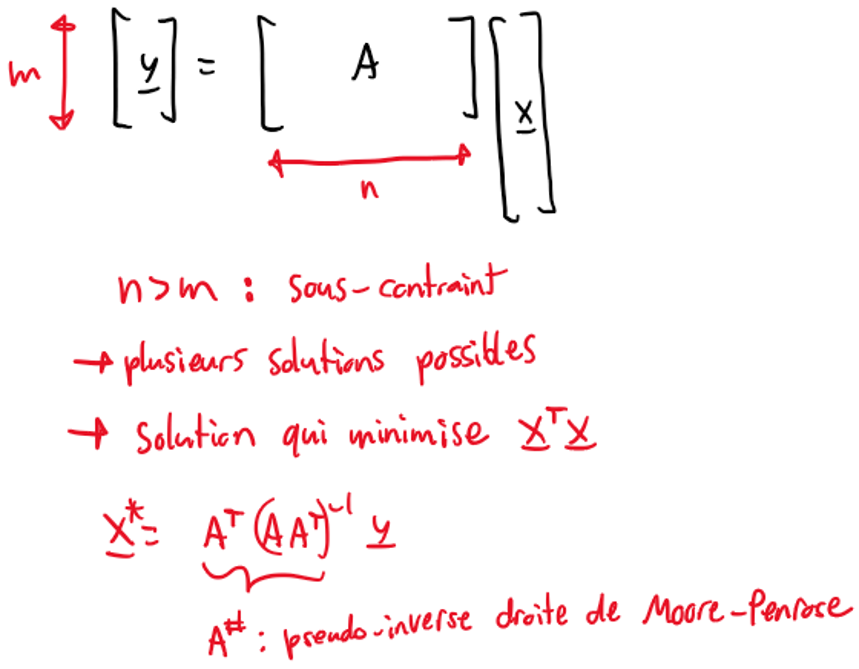
\includegraphics[width=0.75\textwidth]{pseudo-inverse.png}
	\caption{Système sous-contraint - solution avec matrice pseudo-inverse}
	\label{fig:pseudo-inverse}
\end{figure}
%%%%%%%%%%%%%%%%%%%%%%%%%%%%%%%%%%%%%%%%%%%%%%%%%%%%%%%%%%%%



\newpage
\begin{example}[Utilisation d'une matrice pseudo-inverse]
Pour cet exemple, un robot doit produire un force de 14 N sur un mur. Pour y parvenir le courant électrique dans les trois moteurs doit être ajusté. La relation entre la force et le courant dans les moteurs est linéaire et illustrée ci-dessous. On cherche ici une solution qui minimise les pertes joules $ri^2$ dans les moteurs. Comme il y a plusieurs solutions possible pour atteindre le niveau de force désiré, et que la fonction coût à minimiser est quadratique, une matrice pseudo-inverse droite peut être utilisée pour calculer la solution optimale directement, voir Figure \ref{fig:pseudo-inverse-ex1}.
%%%%%%%%%%%%%%%%%%%%%%%%%%%%%%%%%%%%%%%%%%%%%%%%%%%%%%%%%%%%
\begin{figure}[H]
	\centering
		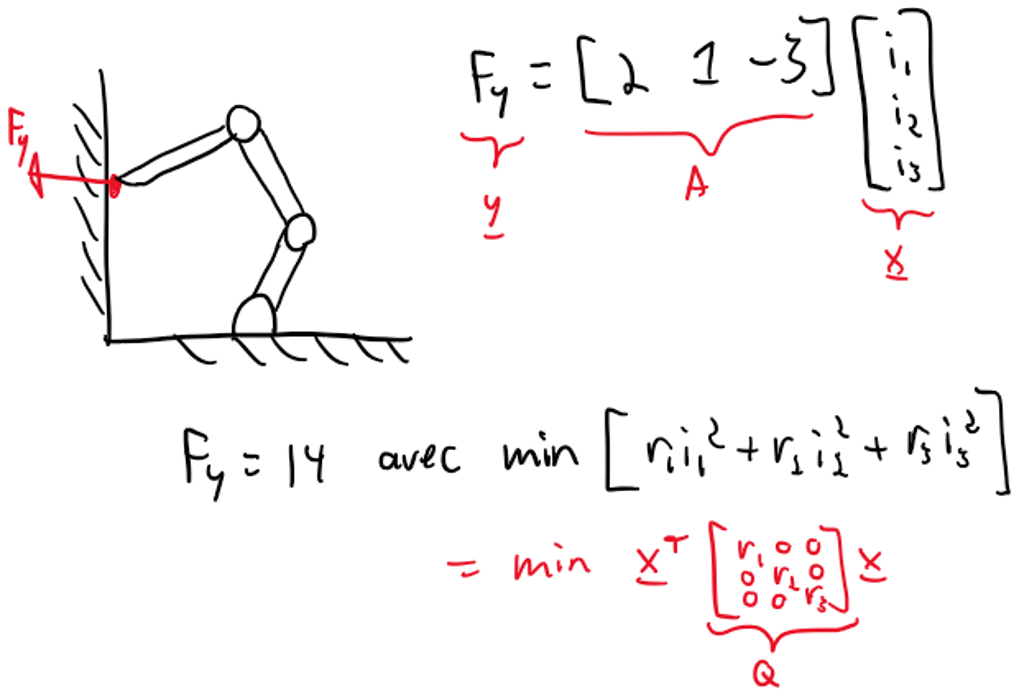
\includegraphics[width=0.7\textwidth]{pseudo-inverse-ex1.png}
		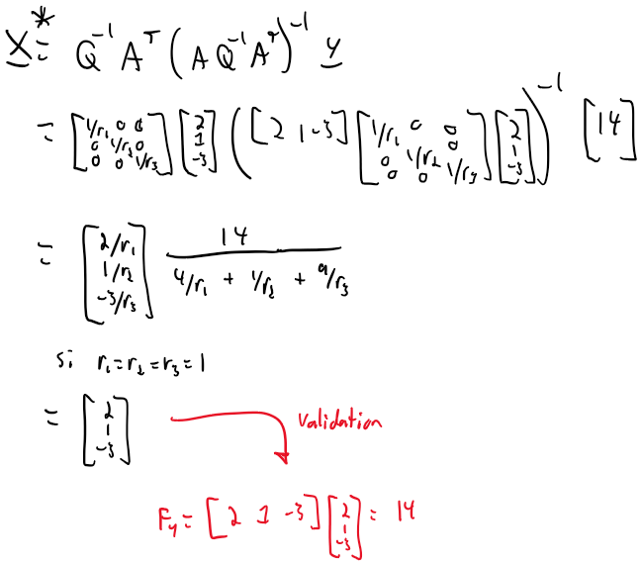
\includegraphics[width=0.5\textwidth]{pseudo-inverse-ex2.png}
	\caption{Exemple d'utilisation d'une matrice pseudo-inverse}
	\label{fig:pseudo-inverse-ex1}
\end{figure}
%%%%%%%%%%%%%%%%%%%%%%%%%%%%%%%%%%%%%%%%%%%%%%%%%%%%%%%%%%%%
\end{example}



\newpage
%%%%%%%%%%%%%%%%%%%%%%%%%%%%%%%%%%%%%%%%%%%%%%%%%%%%%%%%%%%%
\section{Déterminants}
%%%%%%%%%%%%%%%%%%%%%%%%%%%%%%%%%%%%%%%%%%%%%%%%%%%%%%%%%%%%

À venir!

%%%%%%%%%%%%%%%%%%%%%%%%
\begin{align}
det(A) = det(U) = p_1 p_2 ... p_n
\end{align}
%%%%%%%%%%%%%%%%%%%%%%%%

\newpage
%%%%%%%%%%%%%%%%%%%%%%%%%%%%%%%%%%%%%%%%%%%%%%%%%%%%%%%%%%%%
\section{Vecteurs et valeurs propres}
%%%%%%%%%%%%%%%%%%%%%%%%%%%%%%%%%%%%%%%%%%%%%%%%%%%%%%%%%%%%

Pour les matrices carrées ($m=n$), une autre caractéristique utile est l'ensemble de ses vecteurs et valeurs propres. Un vecteur $\col{x}$ est un vecteur propre d'une matrice $A$ si le résultat $\col{y} = A \col{x}$ est parallèle à l'entrée $\col{x}$, autrement dit s'il existe un scalaire $\lambda$ (appelé valeur propre) tel que:
%%%%%%%%%%%%%%%%%%%%%%%%%%%
\begin{align}
A \col{x} = \lambda  \col{x}
\end{align}
%%%%%%%%%%%%%%%%%%%%%%%%%%%

%%%%%%%%%%%%%%%%%%%%%%%%%%%%%%%%%%%%%%%%%%%%%%%%%%%%%%%%%%%%%
\begin{figure}[H]
	\centering
		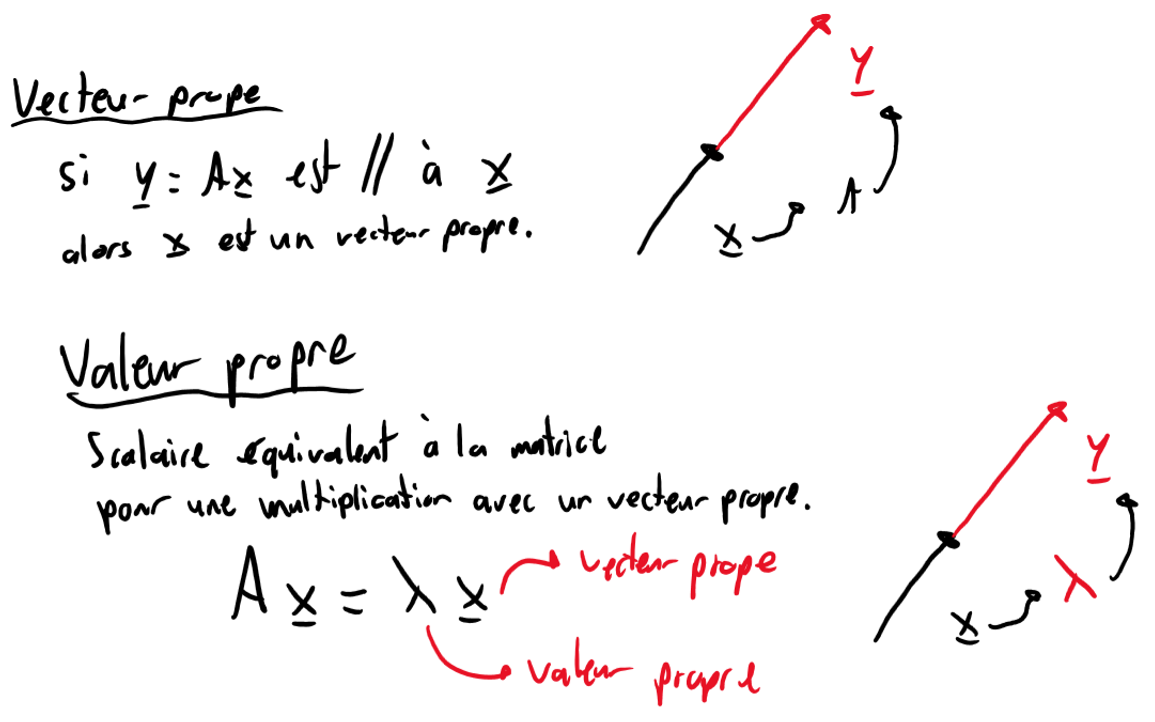
\includegraphics[width=0.85\textwidth]{linalgebra_eigen.png}
	\caption{Vecteurs et valeurs propres}
	\label{fig:eigen}
\end{figure}
%%%%%%%%%%%%%%%%%%%%%%%%%%%%%%%%%%%%%%%%%%%%%%%%%%%%%%%%%%%%%

Une matrice $n \times n$ va avoir $n$ paires de vecteur et valeurs propres (qui peuvent être répété et aussi des nombres complexes). Si une ou plusieurs valeurs propres de la matrice est égale à zéro alors la matrice est singulière et les vecteurs propres associés forme une base de l'espace nul de la matrice. 

La trace d'un matrice est égale à la somme des valeurs propres et le déterminant d'une matrice est égale à la multiplication de toutes les valeurs propres:
%%%%%%%%%%%%%%%%%%%%%%%%%%%
\begin{align}
trace(A) &= \sum_1^n{ \lambda_i } \\
det(A)   &= \prod_1^n{ \lambda_i }
\end{align}
%%%%%%%%%%%%%%%%%%%%%%%%%%%

Pour déterminer les valeurs et vecteurs propres d'une matrice, le problème est posé ainsi:
%%%%%%%%%%%%%%%%%%%%%%%%%%%
\begin{align}
A \col{x} &= \lambda  \col{x} \\
(A - \lambda I) \col{x} &= \col{0}
\end{align}
%%%%%%%%%%%%%%%%%%%%%%%%%%%
La matrice $(A - \lambda I)$ doit être singulière pour qu'il existe des solutions non-nulles à cette équation. Il est donc possible de trouver les valeurs propres $\lambda_i$ en solutionnant l'équation suivante:
%%%%%%%%%%%%%%%%%%%%%%%%%%%
\begin{align}
det(A - \lambda I) = 0
\end{align}
%%%%%%%%%%%%%%%%%%%%%%%%%%%
Pour chaque solution, i.e pour chaque valeur propre $\lambda_i$, il est possible de déterminer le vecteur propre associé $\col{v}_i$ en déterminant l'espace nul de $(A - \lambda I)$:
%%%%%%%%%%%%%%%%%%%%%%%%%%%
\begin{align}
\col{v}_i \in nul(A - \lambda I)
\end{align}
%%%%%%%%%%%%%%%%%%%%%%%%%%%
Il est à noté que pour chaque valeur propre, le vecteur propre n'est pas unique, seule la direction l'est. Si $\col{v}_i$ est un vecteur propre alors tout multiple de lui même est aussi un vecteur propre. Donc autrement dit pour chaque valeur propre $\lambda_i$, on cherche en fait une base pour l'espace 1D associé aux vecteurs propres de cette valeur.



%%%%%%%%%%%%%%%%%%%%%%%%%%%%%%%%%%%%%%%%%%%%%%%%%%%%%%%%%%%%%
\begin{figure}[H]
	\centering
		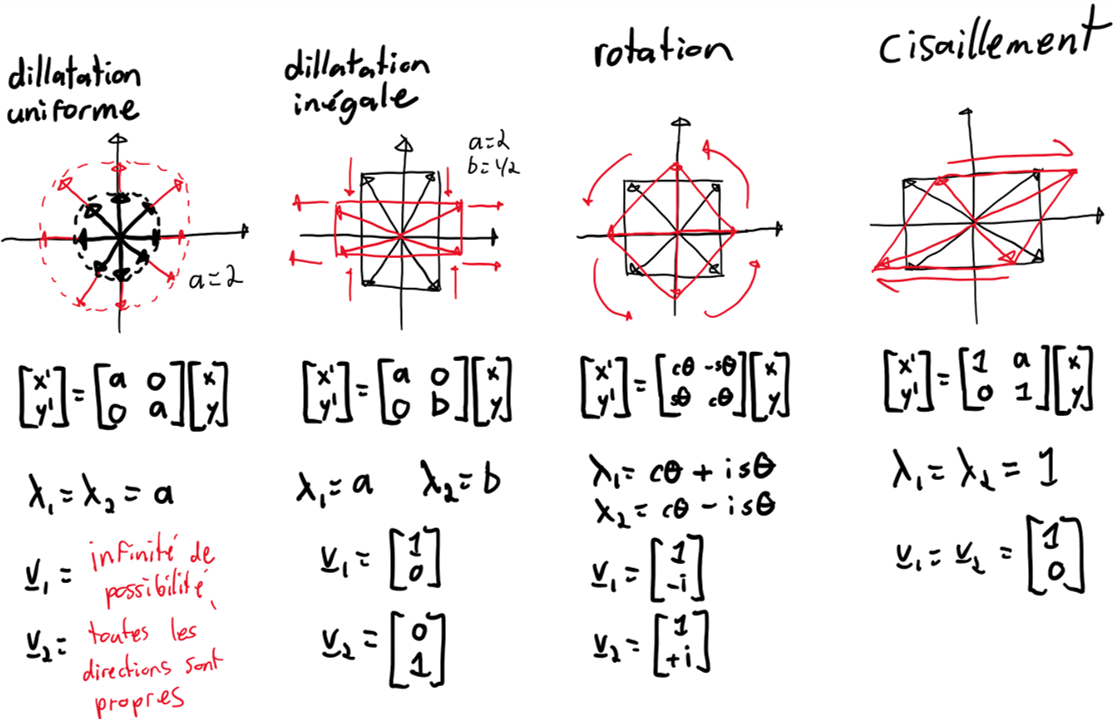
\includegraphics[width=0.95\textwidth]{linalgebra_eigen_exemple.png}
	\caption{Exemple de vecteurs et valeurs propres dans un contexte de transformations géométriques}
	\label{fig:linalgebra_eigen_exemple}
\end{figure}
%%%%%%%%%%%%%%%%%%%%%%%%%%%%%%%%%%%%%%%%%%%%%%%%%%%%%%%%%%%%%

%%%%%%%%%%%%%%%%%%%%%%%%%%%%%%%%%%%%%%%%%%%%%%%%%%%%%%%%%%%%
\subsection{Diagonalisation}
%%%%%%%%%%%%%%%%%%%%%%%%%%%%%%%%%%%%%%%%%%%%%%%%%%%%%%%%%%%%

Si une matrice a $n$ vecteurs propres indépendants, alors la matrice peut être diagonalisée, c'est à dire décomposée sous la forme:
%%%%%%%%%%%%%%%%%%%%%%%%%%%
\begin{align}
A = V \Lambda V^{-1}
\label{eq:diagmatrix}
\end{align}
%%%%%%%%%%%%%%%%%%%%%%%%%%%
où la matrice $V$ regroupe tous les vecteurs propres de $A$, et la matrice diagonale $\Lambda$ toutes les valeurs propres  de $A$:
%%%%%%%%%%%%%%%%%%%%%%%%%%%
\begin{align}
V = 
\left[ \begin{array}{c@{}c@{}c}  
\left[  \begin{array}{c}  \\ \underline{v}_1 \\ \\ \end{array} \right] &  \ldots & \left[  \begin{array}{c} \\ \underline{v}_n \\ \\ \end{array} \right]
\end{array} \right]
\quad \quad
\Lambda = 
\left[ \begin{array}{c c c c}  
\lambda_1 &  0          & 0 & 0 \\
0         &  \lambda_2  & 0      & 0 \\
0         &  0          &\ddots  & 0 \\
0         &  0          & 0  & \lambda_n
\end{array} \right]
\end{align}
%%%%%%%%%%%%%%%%%%%%%%%%%%%

Lorsqu'une matrice a plusieurs vecteur propres associés à la même valeur propre alors la matrice n'est pas diagonalisable. Il est toutefois possible de faire appelle à une méthode alternative appelée la réduction de Jordan. 
%
La diagonalisation d'une matrice peut être interprété comme un changement de base, vers des coordonnées dites propres, pour lesquelles l'effet de la multiplication de cette matrice est indépendant pour chaque axes. 


%%%%%%%%%%%%%%%%%%%%%%%%%%%%%%%%%%%%%%%%%%%%%
\begin{proof}
\label{sec:preuvediag}
%%%%%%%%%%%%%%%%%%%%%%%%%%%%%%%%%%%%%%%%%%%%%

Par définition, si les vecteurs propres $\col{v}_i$ sont multipliés leur matrice $A$, la multiplication est équivalente à les multiplier par les valeurs propres associées $\lambda_i$:
%
%%%%%%%%%%%%%%%%%%%%%%%%%%%
\begin{align}
A V = 
\left[ \begin{array}{c@{}c@{}c}  
A \left[   \begin{array}{c}  \\ \underline{v}_1 \\ \\ \end{array} \right] &  \ldots & \; A \left[  \begin{array}{c} \\ \underline{v}_n \\ \\ \end{array} \right]
\end{array} \right]
= 
\left[ \begin{array}{c@{}c@{}c}  
\lambda_1 \left[   \begin{array}{c}  \\ \underline{v}_1 \\ \\ \end{array} \right] &  \ldots & \;\lambda_n \left[  \begin{array}{c} \\  \underline{v}_n \\ \\ \end{array} \right]
\end{array} \right]
= V \Lambda
\end{align}
\label{eq:diagproof}
%%%%%%%%%%%%%%%%%%%%%%%%%%%
Ensuite, si la matrice $V$ est inversible (ce qui explique la condition d'indépendance des vecteurs propres pour que la matrice soit diagonalisable), il suffit de multiplier l'équation \eqref{eq:diagmatrix} par $V^{-1}$ par la droite pour obtenir l'équation \eqref{eq:diagmatrix}. 
\end{proof}



%%%%%%%%%%%%%%%%%%%%%%%%%%%%%%%%%%%%%%%%%%%%%%%%%%%%%%
\begin{example}[Exemple de diagonalisation pour une dillatation en 2D]
\label{sec:ExempleDeDiagonalisationPourUneDillatationEn2D}
%%%%%%%%%%%%%%%%%%%%%%%%%%%%%%%%%%%%%%%%%%%%%%%%%%%%%%
%%%%%%%%%%%%%%%%%%%%%%%%%%%%%%%%%%%%%%%%%%%%%%%%%%%%%%%%%%%%%
\begin{figure}[H]
	\centering
		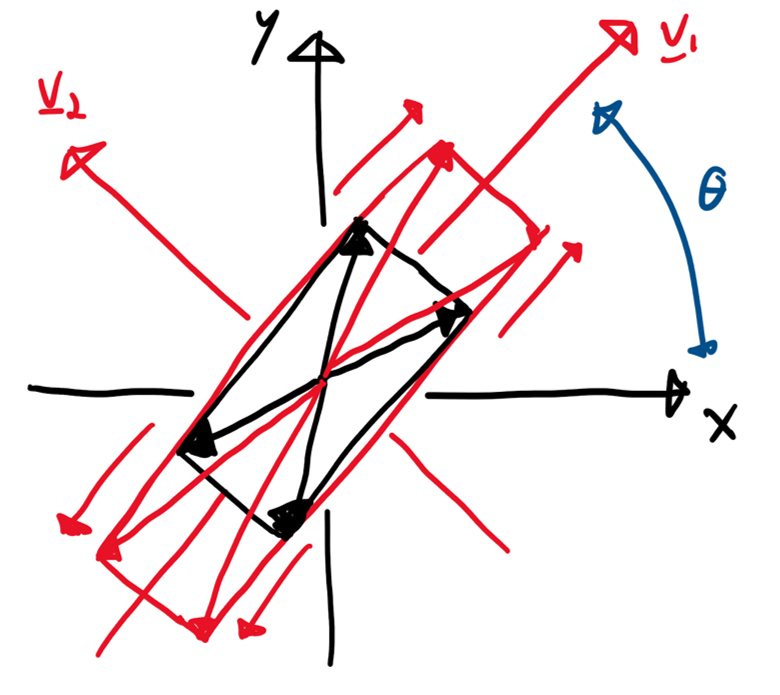
\includegraphics[width=0.35\textwidth]{linalgebra_diag_exemple.png}
	\caption{Exemple de diagonalisation pour une transformation géométrique}
	\label{fig:linalgebra_diag_exemple}
\end{figure}
%%%%%%%%%%%%%%%%%%%%%%%%%%%%%%%%%%%%%%%%%%%%%%%%%%%%%%%%%%%%%

%%%%%%%%%%%%%%%%%%%%%%%%%%%
\begin{align}
A =
\left[ \begin{array}{c c}  
c\theta^2+1     & c\theta s\theta \\
c\theta s\theta & s\theta^2+1
\end{array} \right]
=
\underbrace{
\left[ \begin{array}{c c}  
c\theta & - s\theta \\ 
s\theta &   c\theta 
\end{array} \right]
}_{V}
\;
\underbrace{
\left[ \begin{array}{c c}  
2 & 0 \\
0 & 1 
\end{array} \right]
}_{\Lambda}
\;
\underbrace{
\left[ \begin{array}{c c}  
c\theta &   s\theta \\ 
- s\theta &   c\theta 
\end{array} \right]
}_{V^{-1}}
\end{align}
%%%%%%%%%%%%%%%%%%%%%%%%%%%
\end{example}








%%%%%%%%%%%%%%%%%%%%%%%%%%%%%%%%%%%%%%%%%%%%%%%%%%%%%%%%%%%%
\subsection{Puissance d'une matrice}
%%%%%%%%%%%%%%%%%%%%%%%%%%%%%%%%%%%%%%%%%%%%%%%%%%%%%%%%%%%%

La puissance $p$ d'une matrice est définie comme la multiplication répété de $p$ copie de cette matrice. Si la matrice est diagonalisable, la puissance de la matrice $A$ est égale à
%%%%%%%%%%%%%%%%%%%%%%%%%%%
\begin{align}
A^p = V \Lambda^p V^{-1}
\label{eq:matrixpower}
\end{align}
%%%%%%%%%%%%%%%%%%%%%%%%%%%
avec:
%%%%%%%%%%%%%%%%%%%%%%%%%%%
\begin{align}
\Lambda^p = 
\left[ \begin{array}{c c c c}  
\lambda_1^p t &  0          & 0 & 0 \\
0         &  \lambda_2^p  & 0      & 0 \\
0         &  0          &\ddots  & 0 \\
0         &  0          & 0  & \lambda_n^p
\end{array} \right]
\end{align}
%%%%%%%%%%%%%%%%%%%%%%%%%%

Cette propriété découle de la diagonalisation:
%%%%%%%%%%%%%%%%%%%%%%%%%%%
\begin{align}
A^p = A \; A \; \hdots \; A = V \Lambda V^{-1} \; V \Lambda V^{-1} \;  \hdots \; V \Lambda V^{-1} = V \Lambda \Lambda   \hdots \Lambda V^{-1} = V \Lambda^p V^{-1}
\end{align}
%%%%%%%%%%%%%%%%%%%%%%%%%%%

%%%%%%%%%%%%%%%%%%%%%%%%%%%%%%%%%%%%%%%%%%%%%%%%%%%%%%
\begin{example}[Exemple de calcul de l'évolution d'un système discret]
%%%%%%%%%%%%%%%%%%%%%%%%%%%%%%%%%%%%%%%%%%%%%%%%%%%%%%
La suite de Fibonacci est définie par une séquence de chiffre pour lequel le prochain est la somme des deux précédents:
%%%%%%%%%%%%%%%%%%%%%%%%%%%
\begin{align}
0 \; 1\;1\;2\;3\;5\;8\;13\;21\;34\;55
\end{align}
%%%%%%%%%%%%%%%%%%%%%%%%%%%
Le chiffre suivant est calculé en fonction des deux précédents:
%%%%%%%%%%%%%%%%%%%%%%%%%%%
\begin{align}
f_{k+1} = f_{k} + f_{k-1}
\end{align}
%%%%%%%%%%%%%%%%%%%%%%%%%%%
il faut donc un vecteur d'état $\col{x}$ de deux variable ($f_{k}$ et $f_{k-1}$ ) pour prédire le prochain chiffre. L'évolution du vecteur d'état peut être décrite par l'équation matricielle suivante:
%%%%%%%%%%%%%%%%%%%%%%%%%%%
\begin{align}
\underbrace{
\left[ \begin{array}{c}  
f_{k+1} \\ f_{k}
\end{array} \right]
}_{\col{x}_{k+1}}
=
\underbrace{
\left[ \begin{array}{c c}  
1 & 1 \\ 1 & 0 
\end{array} \right]
}_{A}
\underbrace{
\left[ \begin{array}{c}  
f_{k} \\ f_{k-1}
\end{array} \right]
}_{\col{x}_{k}}
\end{align}
%%%%%%%%%%%%%%%%%%%%%%%%%%%

Il est possible de calculer la valeur future d'une évolution discrète comme celle-ci sans calculer toute la séquence grâce la propriété \eqref{eq:matrixpower}:
%%%%%%%%%%%%%%%%%%%%%%%%%%%
\begin{align}
\col{x}_{k+1} &= A \col{x}_{k} \\
\col{x}_{k+2} &= A \col{x}_{k+1} = A A \col{x}_{k} \\
\col{x}_{k+3} &= A \col{x}_{k+2} = A A A \col{x}_{k} \\
\col{x}_{k+p} &= A^p \col{x}_{k} = V \Lambda^p V^{-1} \col{x}_{k}
\label{eq:discretevolutionpower}
\end{align}
%%%%%%%%%%%%%%%%%%%%%%%%%%%
Pour la suite de Fibonacci, la matrice $A$ qui décrit l'évolution peut être diagonalisée. Premièrement on détermine les valeurs propres:
%%%%%%%%%%%%%%%%%%%%%%%%%%%
\begin{align}
0
=
det(A - \lambda I) 
=
det\left(
\left[ \begin{array}{c c}  
1-\lambda & 1 \\ 1 & -\lambda  
\end{array} \right]
\right)
= 
\lambda^2 - \lambda -1 
\end{align}
%%%%%%%%%%%%%%%%%%%%%%%%%%%
Il y a donc deux solutions:
%%%%%%%%%%%%%%%%%%%%%%%%%%%
\begin{align}
\lambda_1 = \frac{1 + \sqrt{5}}{2} = 1.61803399 \quad\quad \lambda_2 = \frac{1 - \sqrt{5}}{2} = -0.61803399
\end{align}
%%%%%%%%%%%%%%%%%%%%%%%%%%%
ou la première valeur propre est égale au très fameux nombre d'or. Il est possible de déterminer les vecteurs propres associé en substituant dans l'équation $A \col{v} = \lambda \col{v}$, on trouve alors:
%%%%%%%%%%%%%%%%%%%%%%%%%%%
\begin{align}
\col{v}_1 = 
\left[ \begin{array}{c}  
\lambda_1 \\ 1
\end{array} \right]
\quad\quad 
\col{v}_2 = 
\left[ \begin{array}{c}  
\lambda_2 \\ 1 
\end{array} \right]
\end{align}
%%%%%%%%%%%%%%%%%%%%%%%%%%%
Il est donc maintenant possible de calculer n'importe quel position future dans la séquence directement grâce à l'équation \eqref{eq:discretevolutionpower}. Si on cherche la position $p=1E9$ à partir du début de la suite de Fibonacci:
%%%%%%%%%%%%%%%%%%%%%%%%%%%
\begin{align}
\col{x}_{p} &= V \Lambda^p V^{-1} \col{x}_{0} \\
\left[ \begin{array}{c}  
f_p \\ f_{p-1}
\end{array} \right]
&= 
\left[ \begin{array}{c c }  
\lambda_1 & \lambda_2 \\
1         & 1 \\
\end{array} \right]
\left[ \begin{array}{c c }  
\lambda_1^p & 0 \\
0         & \lambda_2^p \\
\end{array} \right]
\left[ \begin{array}{c c }  
\lambda_1 & \lambda_2 \\
1         & 1 \\
\end{array} \right]^{-1} 
\left[ \begin{array}{c}  
1 \\ 0
\end{array} \right]
\end{align}
%%%%%%%%%%%%%%%%%%%%%%%%%%%
lorsque $p$ est très grand il est possible de simplifier le calcul en négligeant la contribution $\lambda_2^p \approx 0$ puisque lorsque que la valeur absolue de la base est inférieur à l'unité, la puissance tend vers zéro lorsque $p$ tend vers l'infini. Il est donc possible de simplifier:
%%%%%%%%%%%%%%%%%%%%%%%%%%%
\begin{align}
\left[ \begin{array}{c}  
f_p \\ f_{p-1}
\end{array} \right]
&= 
\left[ \begin{array}{c c }  
\lambda_1 & \lambda_2 \\
1         & 1 \\
\end{array} \right]
\left[ \begin{array}{c c }  
\lambda_1^p & 0 \\
0         & 0 \\
\end{array} \right]
\frac{1}{\lambda_1 - \lambda_2}
\left[ \begin{array}{c c }  
1 & -\lambda_2 \\
-1         & \lambda_1 \\
\end{array} \right] 
\left[ \begin{array}{c}  
1 \\ 0
\end{array} \right]
\\
\left[ \begin{array}{c}  
f_p \\ f_{p-1}
\end{array} \right]
&= 
\left[ \begin{array}{c c}  
\lambda_1^{p+1} & 0 \\
\lambda_1^{p}  & 0\\
\end{array} \right]
\frac{1}{\lambda_1 - \lambda_2}
\left[ \begin{array}{c }  
1  \\
-1   \\
\end{array} \right] 
\\
\left[ \begin{array}{c}  
f_p \\ f_{p-1}
\end{array} \right]
&= 
\frac{1}{\lambda_1 - \lambda_2}
\left[ \begin{array}{c}  
\lambda_1^{p+1}\\
\lambda_1^{p} \\
\end{array} \right] 
\end{align}
%%%%%%%%%%%%%%%%%%%%%%%%%%% df
Il est donc possible de calculer directement la valeur dans la suite pour une positon $p$ lorsque $p$ est très grand:
%%%%%%%%%%%%%%%%%%%%%%%%%%%
\begin{align}
f_p = \frac{\lambda_1^{p+1}}{\lambda_1 - \lambda_2} = \frac{1.618^{(p+1)}}{\sqrt{5}}
\end{align}
%%%%%%%%%%%%%%%%%%%%%%%%%%%
\end{example}

%%%%%%%%%%%%%%%%%%%%%%%%%%%%%%%%%%%%%%%%%%%%%%%%%%%%%%%%%%%%
\subsection{Exponentiel de matrice}
%%%%%%%%%%%%%%%%%%%%%%%%%%%%%%%%%%%%%%%%%%%%%%%%%%%%%%%%%%%%

À venir!


%%%%%%%%%%%%%%%%%%%%%%%%%%%
\begin{align}
e^{At} = V e^{\Lambda t} V^{-1}
\end{align}
%%%%%%%%%%%%%%%%%%%%%%%%%%%

%%%%%%%%%%%%%%%%%%%%%%%%%%%    
\begin{align}
e^{\Lambda t} = 
\left[ \begin{array}{c c c c}  
e^{\lambda_1 t} &  0          & 0 & 0 \\
0         &  e^{\lambda_2 t}  & 0      & 0 \\
0         &  0          &\ddots  & 0 \\
0         &  0          & 0  & e^{\lambda_n t}
\end{array} \right]
\end{align}
%%%%%%%%%%%%%%%%%%%%%%%%%%

